%===============================================================================
% LaTeX sjabloon voor de bachelorproef toegepaste informatica aan HOGENT
% Meer info op https://github.com/HoGentTIN/bachproef-latex-sjabloon
%===============================================================================

\documentclass{../../Templates/bachproef-tin}

\usepackage{../../Templates/hogent-thesis-titlepage} % Titelpagina conform aan HOGENT huisstijl

%%---------- Documenteigenschappen ---------------------------------------------
% TODO: Vul dit aan met je eigen info:

% De titel van het rapport/bachelorproef
\title{Gedecentraliseerd en transparant versiebeheer aan de hand van blockchain principes en IPFS: een praktische toepassing voor open source bedrijven.}

% Je eigen naam
\author{Michiel Schoofs}

% De naam van je promotor (lector van de opleiding)
\promotor{Karine Samyn}

% De naam van je co-promotor. Als je promotor ook je opdrachtgever is en je
% dus ook inhoudelijk begeleidt (en enkel dan!), mag je dit leeg laten.
\copromotor{Maurice Dalderup}

% Indien je bachelorproef in opdracht van/in samenwerking met een bedrijf of
% externe organisatie geschreven is, geef je hier de naam. Zoniet laat je dit
% zoals het is.
\instelling{---}

% Academiejaar
\academiejaar{2019-2020}

% Examenperiode
%  - 1e semester = 1e examenperiode => 1
%  - 2e semester = 2e examenperiode => 2
%  - tweede zit  = 3e examenperiode => 3
\examenperiode{2}

%===============================================================================
% Inhoud document
%===============================================================================

\begin{document}

%---------- Taalselectie -------------------------------------------------------
% Als je je bachelorproef in het Engels schrijft, haal dan onderstaande regel
% uit commentaar. Let op: de tekst op de voorkaft blijft in het Nederlands, en
% dat is ook de bedoeling!

%\selectlanguage{english}

%---------- Titelblad ----------------------------------------------------------
\inserttitlepage

%---------- Samenvatting, voorwoord --------------------------------------------
\usechapterimagefalse
%%=============================================================================
%% Voorwoord
%%=============================================================================

\chapter*{\IfLanguageName{dutch}{Woord vooraf}{Preface}}
\label{ch:voorwoord}

%% TODO:
%% Het voorwoord is het enige deel van de bachelorproef waar je vanuit je
%% eigen standpunt (``ik-vorm'') mag schrijven. Je kan hier bv. motiveren
%% waarom jij het onderwerp wil bespreken.
%% Vergeet ook niet te bedanken wie je geholpen/gesteund/... heeft

Ik wil graag de volgende personen bedanken:

\begin{enumerate}
\item Karine Samyn voor de begeleiding, constructieve feedback en vooral haar geduld.
\item Maurice Dalderup voor de begeleiding en de rol van co-promotor op te nemen.
\item Ria Schoofs voor het kritisch nalezen.
\item Fatih Mercan for being a good friend and helping me pull through. Hopefully we'll meet one day outside of cyberspace. 
\end{enumerate}

%%=============================================================================
%% Samenvatting
%%=============================================================================

% TODO: De "abstract" of samenvatting is een kernachtige (~ 1 blz. voor een
% thesis) synthese van het document.
%
% Deze aspecten moeten zeker aan bod komen:
% - Context: waarom is dit werk belangrijk?
% - Nood: waarom moest dit onderzocht worden?
% - Taak: wat heb je precies gedaan?
% - Object: wat staat in dit document geschreven?
% - Resultaat: wat was het resultaat?
% - Conclusie: wat is/zijn de belangrijkste conclusie(s)?
% - Perspectief: blijven er nog vragen open die in de toekomst nog kunnen
%    onderzocht worden? Wat is een mogelijk vervolg voor jouw onderzoek?
%
% LET OP! Een samenvatting is GEEN voorwoord!

%%---------- Nederlandse samenvatting -----------------------------------------
%
% TODO: Als je je bachelorproef in het Engels schrijft, moet je eerst een
% Nederlandse samenvatting invoegen. Haal daarvoor onderstaande code uit
% commentaar.
% Wie zijn bachelorproef in het Nederlands schrijft, kan dit negeren, de inhoud
% wordt niet in het document ingevoegd.

\IfLanguageName{english}{%
\selectlanguage{dutch}
\chapter*{Samenvatting}
\lipsum[1-4]
\selectlanguage{english}
}{}

%%---------- Samenvatting -----------------------------------------------------
% De samenvatting in de hoofdtaal van het document

\chapter*{\IfLanguageName{dutch}{Samenvatting}{Abstract}}


%---------- Inhoudstafel -------------------------------------------------------
\pagestyle{empty} % Geen hoofding
\tableofcontents  % Voeg de inhoudstafel toe
\cleardoublepage  % Zorg dat volgende hoofstuk op een oneven pagina begint
\pagestyle{fancy} % Zet hoofding opnieuw aan

%---------- Lijst figuren, afkortingen, ... ------------------------------------

% Indien gewenst kan je hier een lijst van figuren/tabellen opgeven. Geef in
% dat geval je figuren/tabellen altijd een korte beschrijving:
%
%  \caption[korte beschrijving]{uitgebreide beschrijving}
%
% De korte beschrijving wordt gebruikt voor deze lijst, de uitgebreide staat bij
% de figuur of tabel zelf.

\listoffigures
\listoftables

% Als je een lijst van afkortingen of termen wil toevoegen, dan hoort die
% hier thuis. Gebruik bijvoorbeeld de ``glossaries'' package.
% https://www.overleaf.com/learn/latex/Glossaries

%---------- Kern ---------------------------------------------------------------

% De eerste hoofdstukken van een bachelorproef zijn meestal een inleiding op
% het onderwerp, literatuurstudie en verantwoording methodologie.
% Aarzel niet om een meer beschrijvende titel aan deze hoofstukken te geven of
% om bijvoorbeeld de inleiding en/of stand van zaken over meerdere hoofdstukken
% te verspreiden!

%%=============================================================================
%% Inleiding
%%=============================================================================

\chapter{\IfLanguageName{dutch}{Inleiding}{Introduction}}
\label{ch:inleiding}
\subsection{Introductie versiebeheersystemen}
Elke software ontwikkelaar kan beamen dat software fel onderhevig is aan veranderingen. Constant moeten er nieuwe functies worden geïmplementeerd en fouten worden rechtgezet. Dit probleem wordt enkel verergerd indien er tientallen mensen samen aan deze projecten werken. Versiebeheersystemen bieden een oplossing voor deze problemen. Tegenwoordig zijn ze een onmisbaar deel geworden van de manier waarop software wordt ontwikkeld.\\

Deze systemen delen software op in een aaneenschakeling van veranderingen. Deze veranderingen worden ook wel versies genoemd. Deze systemen maken het mogelijk om nieuwe wijzigingen aan te brengen en toegang te krijgen tot oudere versies. Moderne versiebeheersystemen bieden daarbovenop ook de mogelijkheid om twee conflicterende wijzigingen samen te voegen. Hierdoor wordt samenwerken aan grote projecten vergemakkelijkt.\\

Kort samengevat bestaat een versiebeheersysteem uit twee verschillende functies:

\begin{enumerate}
\item Een plaats waar bestanden kunnen worden opgeslagen en opgevraagd worden.
\item Een manier om wijzigingen aan te brengen en toegang te krijgen tot eerdere versies van deze bestanden.
\end{enumerate}

Versiebeheersystemen stellen softwareontwikkelaars instaat om code publiek toegankelijk te maken. Hierdoor kan elke software ontwikkelaar de broncode gaan raadplegen en aanpassen. Een principe dat mooi kadert binnen de zogenaamde Open-Source filosofie. Deze filosofie streeft naar een open en democratische ontwikkeling van software. Hierbij staat samenwerken aan verbeteringen centraal. Software projecten worden aldus aanzien als een gezamenlijk project.

\subsection{Probleem stelling}
Toch is er een probleem met de manier waarop deze systemen functioneren. Ze vereisen namelijk een centrale server voor de bestanden en wijzigingen te gaan opslaan. Dit is problematisch aangezien deze servers eventueel beschadigd of onbereikbaar kunnen zijn. Hierdoor kunnen projecten onbeschikbaar zijn of in het ergste geval zelfs verloren gaan. Dit probleem staat ook wel bekend onder de naam \textbf{Single point of failure}.\\

Een ander probleem is dat deze servers in de handen kunnen komen van grote tech-giganten. Zo heeft Microsoft in 2018 GitHub -een populair versiebeheer platform- overgekocht. Dit druist in tegen de eerder vermelde Open-Source filosofie. Want deze systemen zijn niet gevrijwaard van commerciële invloeden.\\

\subsection{Introductie decentralisatie}

Toch is het door middel van nieuwe technologie zoals Blockchain en IPFS perfect mogelijk om gangbaar alternatief te ontwikkelen zonder dat daar een derde partij bij hoeft betrokken te worden.


\section{\IfLanguageName{dutch}{Onderzoeksvraag}{Research question}}
\label{sec:onderzoeksvraag}
De onderzoeksvraag luidt dus als volgt: \textbf{Hoe kan men doormiddel van Blockchain principes en IPFS een volledig en transparant versiebeheersysteem bekomen?}


\section{\IfLanguageName{dutch}{Onderzoeksdoelstelling}{Research objective}}
\label{sec:onderzoeksdoelstelling}

De doelstelling van deze bachelorproef is om een werkend proto-type te ontwerpen dat voldoet aan onderstaande criteria:

\begin{enumerate}
	\item De oplossing die wordt ontwikkeld mag geen centrale component hebben en moet op een volledig gedistribueerde manier in staat zijn om te functioneren.
	\item De oplossing moet een gebruiker instaat stellen om documenten met anderen te kunnen delen.
	\item De oplossing moet een manier aanbieden om wijzigingen aan deze documenten op te slaan onder de vorm van verschillende versies. Deze verschillende versies moeten kunnen geraadpleegd worden.
\end{enumerate}

Wat is het beoogde resultaat van je bachelorproef? Wat zijn de criteria voor succes? Beschrijf die zo concreet mogelijk. Gaat het bv. om een proof-of-concept, een prototype, een verslag met aanbevelingen, een vergelijkende studie, enz.

\section{\IfLanguageName{dutch}{Opzet van deze bachelorproef}{Structure of this bachelor thesis}}
\label{sec:opzet-bachelorproef}

% Het is gebruikelijk aan het einde van de inleiding een overzicht te
% geven van de opbouw van de rest van de tekst. Deze sectie bevat al een aanzet
% die je kan aanvullen/aanpassen in functie van je eigen tekst.

De rest van deze bachelorproef is als volgt opgebouwd:

In Hoofdstuk~\ref{ch:stand-van-zaken} wordt een overzicht gegeven van de stand van zaken binnen het onderzoeksdomein, op basis van een literatuurstudie.

In Hoofdstuk~\ref{ch:methodologie} wordt de methodologie toegelicht en worden de gebruikte onderzoekstechnieken besproken om een antwoord te kunnen formuleren op de onderzoeksvragen.

% TODO: Vul hier aan voor je eigen hoofstukken, één of twee zinnen per hoofdstuk

In Hoofdstuk~\ref{ch:conclusie}, tenslotte, wordt de conclusie gegeven en een antwoord geformuleerd op de onderzoeksvragen. Daarbij wordt ook een aanzet gegeven voor toekomstig onderzoek binnen dit domein.
\chapter{\IfLanguageName{dutch}{Stand van zaken}{State of the art}}
\label{ch:stand-van-zaken}
\graphicspath{{../../Images/}} 
% Tip: Begin elk hoofdstuk met een paragraaf inleiding die beschrijft hoe
% dit hoofdstuk past binnen het geheel van de bachelorproef. Geef in het
% bijzonder aan wat de link is met het vorige en volgende hoofdstuk.

% Pas na deze inleidende paragraaf komt de eerste sectiehoofding.

%%Dit hoofdstuk bevat je literatuurstudie. De inhoud gaat verder op de inleiding, maar zal het onderwerp van de bachelorproef *diepgaand* uitspitten. De bedoeling is dat de lezer na lezing van dit hoofdstuk helemaal op de hoogte is van de huidige stand van zaken (state-of-the-art) in het onderzoeksdomein. Iemand die niet vertrouwd is met het onderwerp, weet nu voldoende om de rest van het verhaal te kunnen volgen, zonder dat die er nog andere informatie moet over opzoeken \autocite{Pollefliet2011}.

%%Je verwijst bij elke bewering die je doet, vakterm die je introduceert, enz. naar je bronnen. In \LaTeX{} kan dat met het commando \texttt{$\backslash${textcite\{\}}} of \texttt{$\backslash${autocite\{\}}}. Als argument van het commando geef je de ``sleutel'' van een ``record'' in een bibliografische databank in het Bib\LaTeX{}-formaat (een tekstbestand). Als je expliciet naar de auteur verwijst in de zin, gebruik je \texttt{$\backslash${}textcite\{\}}.
%%Soms wil je de auteur niet expliciet vernoemen, dan gebruik je \texttt{$\backslash${}autocite\{\}}. In de volgende paragraaf een voorbeeld van elk.

%%\textcite{Knuth1998} schreef een van de standaardwerken over sorteer- en zoekalgoritmen. Experten zijn het erover eens dat cloud computing een interessante opportuniteit vormen, zowel voor gebruikers als voor dienstverleners op vlak van informatietechnologie~\autocite{Creeger2009}.
%\newpage
\section{Versiebeheer}
\subsection{Inleiding}
\label{sec:vb_inleiding}
Versiebeheer is een belangrijk concept binnen softwareontwikkeling. Zo waren er in 2018 in het  totaal 100 miljoen projecten op het populaire versiebeheer platform GitHub \autocite{Git2018}. GitHub (sinds 2018 overgenomen door Microsoft) is niet de enige speler op de markt. Er zijn ook nog Code Commit van Amazon en GitLab. Veel bedrijven spelen dus in op de behoefte aan een duidelijk en efficiënt versiebeheersysteem. De vraag stelt zich dan ook: welke behoefte lossen deze systemen op?

Stel volgende scenario voor: Alice en Bob zijn aangenomen om te werken voor bedrijf X. Hun eerste taak is een website ontwikkelen. Ze leggen samen alle vereisten vast, bespreken de verschillende technologieën en gaan aan de slag. Op het einde van de eerste dag hebben ze elk een verschillende pagina gemaakt die ze graag met elkaar delen willen delen. Dit kan door bijvoorbeeld via mail de bestanden door te sturen. Een andere mogelijkheid is de bestanden via fysieke hardware zoals een USB-Stick aan elkaar te geven. Het nadeel is dat de code op twee verschillende plaatsen verspreid zit. Als Bob de code kwijt raakt dan zal deze opnieuw moet worden geschreven. Om dit probleem te voorkomen kan men het project op een centrale server opslaan. Bob en Alice zullen hun veranderingen opslaan op deze centrale server. Zo hebben ze altijd toegang tot elkaars werk. 

Deze manier van werken heeft nadelen. Alice kan per ongeluk een bestand overschrijven of een stuk code verwijderen. Tenzij er back-ups zijn is het originele bestand verloren. Om dit probleem te omzeilen wordt er gebruik gemaakt van het concept van \textbf{versies}. Elke aanpassing die er gemaakt wordt resulteert in een nieuwe versie van het project. Men kan altijd terugkeren naar een eerdere versie. Als Alice dus het stukje code verwijdert in versie 15 kan men terug naar versie 14.

\textcite{Loeliger2009} stelt dat een versiebeheersysteem een middel is om verschillende versies van code te beheren en bij te houden. De auteur onderscheidt volgende drie eigenschappen waaraan dergelijke systemen voldoen:

\begin{itemize}
	\item er wordt gebruik gemaakt van een centraal archief. Binnen dit archief worden alle versies van het project bewaard en bijgewerkt.
	\item het centraal archief geeft toegang tot eerdere versies van het project.
	\item alle veranderingen die worden aangebracht aan het archief worden genoteerd in een centraal logboek.
\end{itemize}

Versiebeheer is geen nieuw concept. Er zijn zoals eerder aangehaald verschillende software oplossingen beschikbaar. Volgens \textcite{Chacon2014} zijn er drie grote categorieën (zie \ref{fig_types_cvs} voor een grafische weergave):

\begin{itemize}
	\item lokale versiebeheersystemen: het centraal archief waar de veranderingen in worden bewaard, staat op een lokale computer. Het grootste voordeel is dat een lokaal systeem zeer makkelijk te onderhouden is en eenvoudig op te stellen. Toch is het niet geschikt om bestanden met elkaar te  delen of samen aan bestanden te werken. Een gekend voorbeeld is RCS (Revision Control System) - zie \ref{sec:RCS} -. \\
	
	\item CVCS: om samen te kunnen werken aan dezelfde bestanden kan een CVCS (Centralised Version Control System) worden gebruikt. In plaats van het archief lokaal bij te houden wordt er gebruik gemaakt van een centrale server. Bestanden worden vervolgens lokaal gekopieerd. Als er veranderingen worden aangebracht zullen deze worden doorgestuurd naar de server.Doordat men verplicht is om de bestanden op een centrale plaats af te halen, kan men deze afschermen. Zo kan men de toegang beperken tot enkel de nodige bestanden per gebruiker. \\
	
Een neveneffect van alles centraal te beheren is het zogenaamde \textit{single point of failure (SPOF)} probleem. Een SPOF is een onderdeel van een systeem dat mocht het uitvallen heel het systeem tot een halt roept. Met andere woorden valt het centraal archief weg heeft niemand nog toegang tot het project. Een mogelijke oplossing voor dit probleem is redundantie. Dit betekent het aanbieden van kopieën. \autocite{Sun2007}\\

	\item DVCS: om het SPOF probleem te voorkomen kan men kopieën maken van het centraal archief. Deze kopieën kunnen vervolgens worden verspreid over verschillende computers. Dit is het uitgangspunt van DVCS (Distributed version control System). Elke gebruiker heeft een lokale kopie van de centrale server. De veranderingen aan de bestanden worden eerst aangebracht in het lokaal archief en vervolgens gesynchroniseerd met de centrale variant.\\

Mocht het centraal aanspreekpunt niet beschikbaar zijn is dit geen probleem. Elke gebruiker heeft immers een volledige back-up van het volledige project. In theorie kan de gebruiker zelfs optreden als nieuwe centrale server.
\end{itemize}


\begin{figure}[h!]
	\centering
	\begin{subfigure}[b]{.5\textwidth}
	\centering
		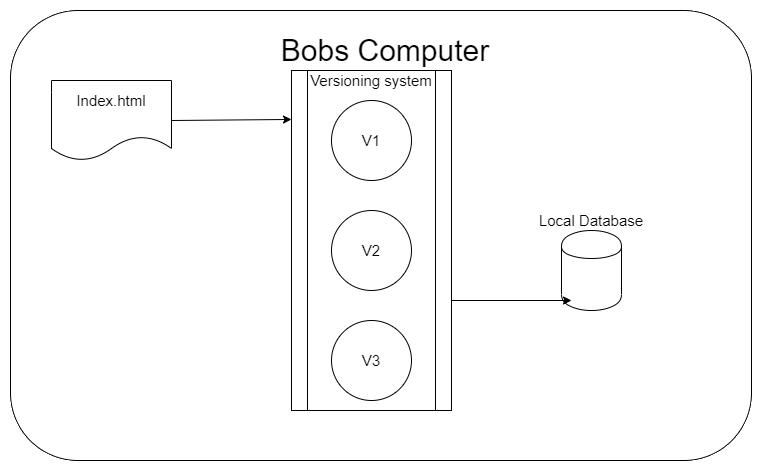
\includegraphics[scale=.3]{LVCS.png}
		\caption[Overzicht structuur Lokale VCS]{Overzicht van de structuur van een Lokale VCS.}
	\end{subfigure}%
	\begin{subfigure}[b]{.5\textwidth}
	\centering
		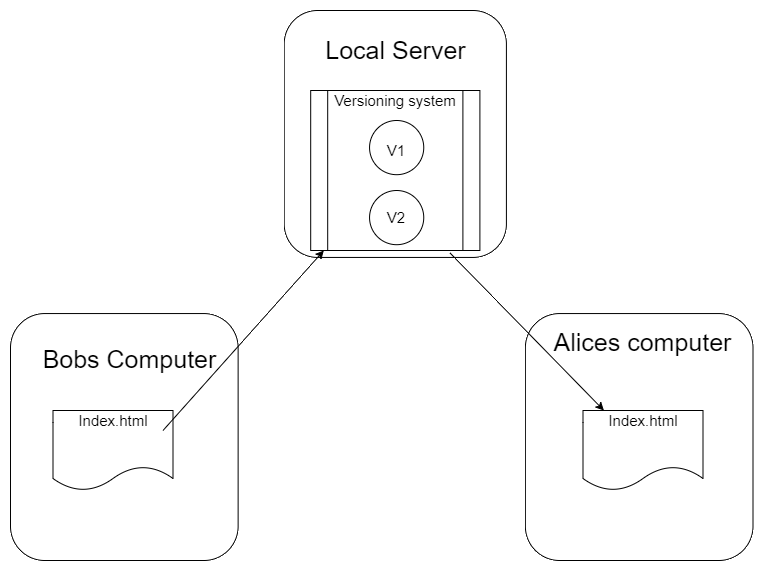
\includegraphics[scale=.3]{CVCS.png}
			\caption[Overzicht structuur CVCS]{Overzicht van de structuur van een CVCS.}
	\end{subfigure}%
	\hfill
	\begin{subfigure}{.5\textwidth}
		\centering
		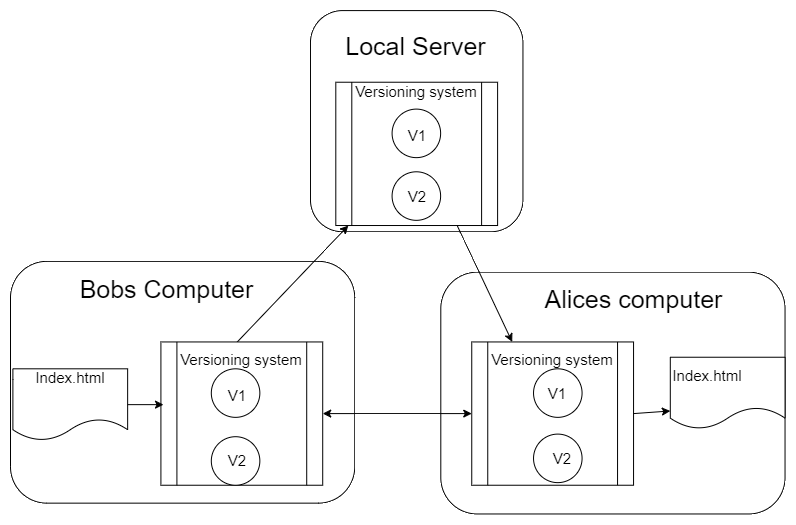
\includegraphics[scale=0.3]{DVCS.png}
	\caption[Overzicht structuur DVCS]{Overzicht van de structuur van een DVCS.}
	\end{subfigure}
	
	\caption[Overzicht types VCS]{Overzicht van de drie types van VCS zoals aangegeven door \textcite{Chacon2014}.}\label{fig_types_cvs}
\end{figure}

	
\subsection{RCS}
\label{sec:RCS}


RCS \textit{(Revision Control System)} is een lokaal versiebeheer systeem. Het wordt voor het eerst beschreven in een artikel geschreven door \textcite{Tichy85rcs}. Het werd verder ontwikkeld binnen het GNU project -Een open source besturingssysteem \footnote{GNU is veel meer dan enkel open source. Het GNU project is sterk verbonden met de ideologie en organisatie van de free software foundation (FSF). Meer informatie omtrent deze organisatie en beweging is te vinden op: \url{https://www.fsf.org/}}- waar het als vervanging voor het CSSC Systeem \autocite{GNUCSSC} werd gebruikt. CSSC is een systeem gebaseerd op SCCS (Source code control system) dat ontworpen is voor UNIX systemen. SCCS is in opdracht van Bell Labs ontwikkeld door \textcite{Rochkind1975}.\\

Voordat RCS op de markt kwam is er nog tal van andere software ontwikkeld. Zo was er CA-Panvalet een gepatenteerde oplossing voor Mainframe computers.\\

Waarom is het interessanter om RCS in detail te bekijken? Veel van de concepten waar het gebruik van maakt zijn aanwezig in moderne systemen (zoals GIT). Het is open source en wordt nog steeds op vrijwillige basis onderhouden, wat aansluit bij de visie van deze bachelorproef.\\

De manier waarop versies worden bijgehouden in RCS -zoals door \textcite{Tichy85rcs} beschreven- is gebaseerd op een boomstructuur -denk aan een stamboom-. Volgens \textcite{Lievens2019}, is een boom een collectie van \textbf{toppen} \textit{(in het Engels ook wel Nodes genoemd)}. Deze toppen hebben een hiërarchische verband.Zo bestaat er bijvoorbeeld een kind-ouder verband. Er zijn twee bijzondere toppen in een boom:

\begin{itemize}
	\item de wortel(\textit{root}): Deze top ligt helemaal aan het begin van de boom. Alle andere toppen zijn afstammelingen van deze top. Het heeft aldus geen ouders.
	\item een blad(\textit{leaf}): Deze top heeft geen kinderen. In tegenstelling tot een wortel kunnen er meerdere bladeren aanwezig zijn.
\end{itemize}

Alle andere toppen worden intermediair genoemd. Elke top heeft mogelijk een aantal kinderen. De diepte van de wortel is nul ($d$=1) en elk kind heeft als diepte: Elk van deze kinderen is op zijn beurt de wortel voor een nieuwe deelboom. Het concept van \textbf{diepte} is belangrijk. 

\begin{equation}
	d_{kind} = d_{ouder} + 1
\end{equation}

%vervang met referentie
Al deze concepten worden ook nog eens grafisch verduidelijkt in de figuur \ref{fig_tree}.

\begin{figure}[h!]
\centering
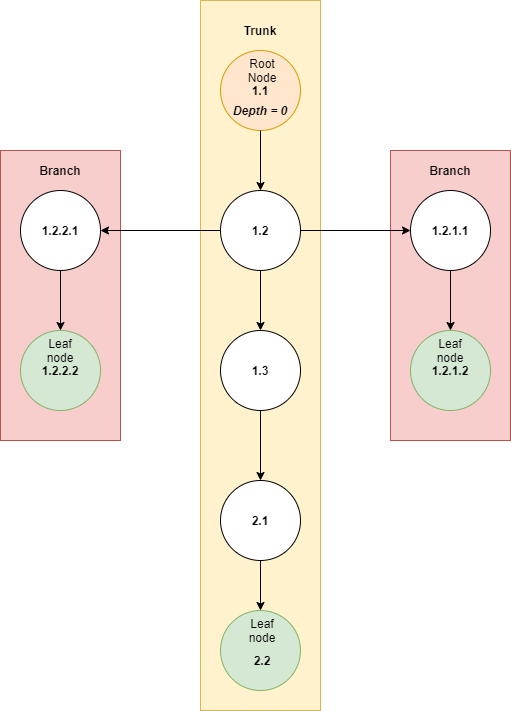
\includegraphics[scale=0.5]{tree1.png}
\caption[Overzicht concepten boomstructuur]{Een overzicht van alle concepten binnen een boomstructuur waar RCS van gebruik maakt.}\label{fig_tree}
\end{figure}

Er kan gebruik gemaakt worden van een boomstructuur om de onderlinge relaties tussen de versies weer te geven. Stel: Bob en Alice zijn bezig aan de hoofdpagina. Bob maakt een initiële versie van de pagina. Vervolgens wilt hij die graag delen met Alice. Hiervoor gebruikt hij het commando om een nieuwe versie aan te maken\footnote{\Verb+ci homepage.html+}. Dit commando wordt \textbf{inchecken} genoemd. Binnen GIT is dit vergelijkbaar met het commando \textit{git push}. Aangezien dit de eerste versie is kan men dit vergelijken met het aanmaken van een wortel. Volgende versies worden kinderen van de vorige versie. Zo wordt versie 1.4 kind van versie 1.3. Inchecken gaat niet alleen onze boomstructuur aanmaken maar ook de extensie \textit{.v} toevoegen (\verb+homepage.html.v+). Het originele bestand wordt ook verwijderd\\

Het bestand krijgt ook een \textbf{versienummer}. Dit versienummer heeft de vorm: $x_1.x_2$.\ $x_1$ (ook wel \textit{release} genoemd) staat voor een grote verandering. Bijvoorbeeld het in productie nemen van een nieuwe versie.$x_2$ (\textit{level}) staat voor een kleinere verandering. Een andere manier om $x_2$ te bekijken is de diepte met als wortel de laatste release ($x_1$). 1.1 is het versienummer van de wortel die Bob heeft aangemaakt. 1.4 is het derde kind van de wortel.Elke check-in zal het level ($x_2$) met één verhogen. Het release nummer ($x_1$) wordt manueel verhoogd door middel van de \textit{-r} optie bij check-in \footnote{\Verb+ci -r2 homepage.html+}. Bij branches is er ook nog spraken van $x_3$ en $x_4$ zie \ref{par:branches}.\\

Deze manier van versies te bestempelen wordt nog steeds gebruikt. Het is echter niet de enige manier. \textit{Semantic versioning} is een gekend alternatief. Het concept van versienummers bestaat in Git onder de vorm van \textit{tags} (\ref{sec:GIT}).\\

Er is nu een bestand onder de vorm \verb+homepage.html.v+. Hoe kan Alice nu dit bestand aanpassen en een nieuwe versie publiceren? Alice zal het bestand moeten \textbf{uitchecken}.Dit kan ze doen door middel van het commando \verb+co+ en de naam van het bestand \footnote{(\Verb+co homepage.html+)} . Het uitchecken is aldus het verkrijgen van een specifieke versie uit het archief. Als er geen specifieke versie wordt meegegeven wordt de laatste versie opgehaald. Om een specifieke versie op te halen kan er gebruik gemaakt worden van de optie -r  \footnote{(\Verb+co -r1.1 homepage.html+)} . Alice heeft nu een kopie van het originele bestand gekregen. Merk op dat in tegenstelling tot inchecken ons archief niet wordt verwijderd. Vervolgens kan ze in deze lokale kopie wijzigingen aanbrengen. Tot slot wordt het bestand weer aan het lokaal archief toegevoegd door middel van inchecken. Het equivalent van \verb+co+ binnen git is \verb+git pull+.\\

\begin{wrapfigure}{r}{0.5\textwidth}
\begin{center}
  	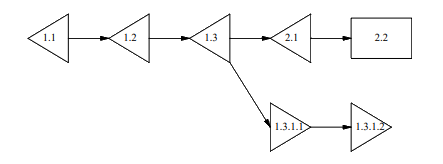
\includegraphics[scale=0.6]{deltas.png}
\end{center}
\caption[Voorbeeld van deltas.]{Een voorbeeld van deltas.De Trunk bevat een series van achterwaardse deltas terwijl alle branches enkel voorwaardse deltas bevatten. Grafiek afkomstig uit \textcite{Tichy85rcs}}\label{fig_deltas}
\end{wrapfigure}

Hoe worden de verschillen tussen de versies bijgehouden in ons lokaal archief? Een mogelijke oplossing zou zijn om alle versies van het bestand afzonderlijk bij te houden. Dit vraagt veel opslagruimte. RCS gebruikt voor dit probleem het concept van \textbf{deltas}. Een delta houdt bij welke regels veranderd zijn ten opzichte van de vorige versie. Doordat de delta enkel de relevante lijnen bijhoudt wordt de opslag beperkt \footnote{De delta wordt opgebouwd aan de hand van het GNU commando diff \url{https://www.gnu.org/software/diffutils/}}. Er zijn twee types van deltas: \textbf{voorwaardse deltas} en \textbf{achterwaardse deltas}. Bij het inchecken van een nieuwe versie zal de vorige versie worden vervangen door een achterwaardse delta. Zit men momenteel op versie 1.3 en  vraagt men versie 1.2 dan zal de achterwaardse delta van versie 1.2 worden toegepast op versie 1.3. (Voorwaardse deltas komen aan bod in het gedeelte over branching (\ref{par:branches}). Het concept van deltas wordt nog eens verduidelijkt door een voorbeeld in de appendix -zie \ref{ch:voorbeeld-rcs}-.)\\

Inchecken en uitchecken ligt aan de basis van het archiefsysteem. Toch is er nog een probleem aanwezig met deze manier van werken. Stel dat Alice en Bob gelijktijdig wijzigingen aanbrengen aan een bestand. Ze willen dit bestand elk afzonderlijk publiceren.  Hierdoor ontstaan er twee versies die afstammen van één gezamenlijke versie. De boomstructuur wordt in twee gesplitst. Dit is niet mogelijk aangezien een versie altijd uniek moet zijn. Hoe kan men verzekeren dat elke versie slechts één kind heeft (op dezelfde branch)? Dit probleem wordt opgelost door \textbf{sloten}(engels=lock).Dit concept geeft gebruikers de mogelijkheid om een versie te  versleutelen. Terwijl een versie versleuteld is kan niemand anders wijzigingen aanbrengen. Andere gebruikers kunnen deze nog bekijken. Op het moment dat Bob zijn versie gaat uitchecken kan hij deze versleutelen (door middel van de \textit{-l} optie bij het co commando). Hierdoor kan Alice geen nieuwe versie meer aanmaken tot Bob zijn wijzigingen heeft doorgevoerd. Met andere woorden zolang Bob het slot niet vrijgeeft kunnen er geen nieuwe versies worden aangemaakt\footnote{In sommige gevallen kan het slot ook worden 'geforceerd' mocht Bob bijvoorbeeld ziek vallen}. Deze manier van werken heeft een zichtbaar nadeel. Alice is verplicht om te wachten op Bobs nieuwe versie alvorens ze veranderingen kan aanbrengen. Git gebruikt het concept van sloten niet. Daar maakt men gebruik van \textbf{merges} om dit zelfde probleem aan te pakken %\ref{sec:GIT}%.

\subsubsection{Opmerkingen}
In het originele artikel wordt de klemtoon gelegd op het onderling delen van de verschillende versies. Hierdoor kan men de indruk krijgen dat er een centrale server betrokken is. Dit is niet het geval. De software is ontworpen om op één besturingssysteem uitgevoerd te worden. Volgens \textcite{Debian2020} is GNU aangezien het gebaseerd is op UNIX een \textit{multi-user os}. Dat wil zeggen dat meerdere gebruikers het systeem tezelfdertijd kunnen gebruiken door middel van een terminal connectie. Hierdoor kan men onderling de bestanden delen ondanks dat men niet gaat werken in een CVCS.

\subsection{branches}
\label{par:branches}
\subsubsection{Duiding}
Door het principe van sloten en inchecken lijkt het alsof elke versie exact één opvolger heeft. Zo zal versie 1.3 de opvolger zijn van 1.2. Toch kunnen er zich zoals in een stamboom  vertakkingen voordoen. De vertakkingen worden \textbf{Branches} genoemd. De hoofdboom (niet vertakte toppen die afstammen van de wortel) wordt de \textbf{trunk} genoemd. Dit principe kan men het best demonstreren aan de hand van een figuur. Zo kan men zien in figuur \ref{fig_tree} dat er twee vertakkingen zijn op versie 1.2. Het principe van vertakkingen lijkt op het eerste zicht complex en onoverzichtelijk. \textcite{Tichy85rcs} geeft enkele redenen om dit toch toe te passen.

\begin{enumerate}
\item Doorvoeren van veranderingen in oude versies: Stel dat een bedrijf een oude versie van een software product gebruikt. Dit product is ontwikkeld met behulp van RCS. Er wordt een fout in deze oude versie gevonden die om een oplossing vraagt. Aangezien er in de tussentijd nieuwere versies zijn is dit niet evident. Het bedrijf zou volledig moeten overstappen op de nieuwste versie alvorens een aanpassing kan gebeuren. Om deze situatie te vermijden kan men gebruik maken van vertakkingen. Zo kan men een vertakking maken op de gewenste versie en kleine aanpassingen doorvoeren.\\
\item Andere implementaties: stel dat een ontwikkelaar een nieuw stuk code wilt uittesten. Deze heeft niet het gewenste resultaat. Mocht dit stuk code bewaard worden op de hoofdboom (\textit{trunk}) dan is er een onstabiele versie gepubliceerd. Een gebruiker die op dat moment de recentste versie opvraagt, krijgt dus een niet werkend product.\\
Door branches te gebruiken kan men ervoor zorgen dat er enkel werkende versie op de hoofdboom terecht komen. Nieuwe stukken code worden eerst geïsoleerd en getest alvorens opgenomen te worden. Op die manier blijft het archief in een overzichtelijke en stabiele vorm.
\end{enumerate}

\begin{wrapfigure}{L}{0.5\textwidth}
\begin{center}
  	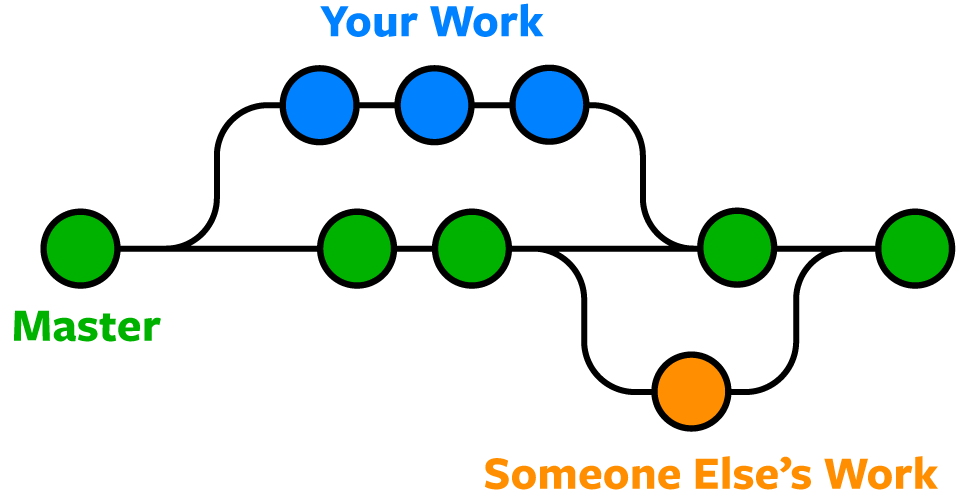
\includegraphics[scale=0.2]{git-branches-merge.png}
\end{center}
\caption[Voorbeeld merge proces.]{Een voorbeeld van een merge proces. Eerst wordt er een branch aangemaakt die na drie versies terug in de master wordt gemerged. Grafiek gepubliceerd door \textcite{NobleDesktop2018}}\label{fig_merge}
\end{wrapfigure}

Door middel van vertakkingen kan code worden geschreven en de hoofdboom stabiel gehouden. Zelfs met veel ontwikkelaars en grote projecten kan men door deze manier van werken code conflicten vermijden. Eenmaal de code klaar is voor productie kan men deze gaan publiceren op de hoofdboom. Dit concept wordt ook wel \textbf{mergen} genoemd. Dit principe wordt geïllustreerd door de figuur \ref{fig_merge}.

%todo uitleg van RCS branching en forward deltas

\subsubsection{Flows}
Er is echter nog een grote vraag die niet beantwoord is: wanneer moet men gaan vertakken?

De eerste reden aangehaald door \textcite{Tichy85rcs} -het doorvoeren van veranderingen- is minder relevant binnen de context van DVCS. Er wordt namelijk niet meer op een gezamenlijk archief gewerkt maar op een lokale kopie. Het bedrijf kan dus op zijn eigen kopie lokaal veranderingen aanbrengen .De tweede reden is echter wel belangrijk. Stel dat een project honderden bestanden en ontwikkelaars heeft. In zo een omgeving kunnen veranderingen soms onvoorspelbare gevolgen hebben. Ontwikkelaars kunnen het project vertakken, wijzigen en testen alvorens het in productie te nemen. Dit is het principe achter \textbf{feature branches}.\\

%Voeg meer bron vermeldingen toe

Bij grote software projecten loopt men het risico dat er veel aftakkingen worden gemaakt die niet worden gebruikt (\textbf{branchmania}). Het artikel van \textcite{Bird2012}, benadrukt het belang van levende takken. Dit zijn vertakkingen die actief wordt gebruikt. Dit kan enkel bereikt worden via een duidelijke werkwijze. Deze werkwijze om het aantal vertakkingen zo klein mogelijk te houden wordt geïllustreerd in figuur \ref{fig_mic_flow}.

\begin{figure}
\begin{center}
  	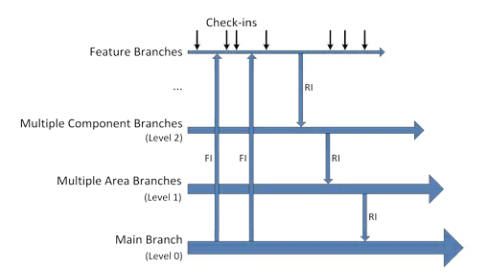
\includegraphics[scale=1]{microsoft-branching.png}
\end{center}
\caption[Voorbeeld flow]{Flow zoals vermeld in het artikel van  \textcite{Bird2012}}\label{fig_mic_flow}
\end{figure}

Elke ontwikkelaar schrijft zijn code op een feature branch. Het risico hiervan is dat men op den duur niet meer compatibel is met de hoofdboom. Er kunnen sinds de vertakking immers verschillende andere versies gepubliceerd zijn. Daarom wordt gewerkt met twee tussenbranches. Hier test men of de code compatibel is met de verschillende andere onderdelen van de software. Het proces waarbij men feature branches integreert in andere tussenbranches noemt men ook wel \textbf{Reverse integration} -aangeduid als RI op de figuur-. Een ander principe dat gebruikt wordt is dat van \textbf{Forward integration}. Hierbij worden de nieuwe versies van de hoofdbranch (ook wel master genoemd) geplaatst op de feature branch. Zo blijft de feature branch compatibel met alle veranderingen.

%toevoegen van GIT Flow
%toevoegen van Trunk based developmet
Buiten de methodiek voorgesteld door \textcite{Bird2012} bestaat er ook GIT Flow en Trunk based development. 


%\subsection{GIT}
%\label{sec:GIT}

\subsection{Conclusie}
\label{vb_conclusie}
De verschillende types van versiebeheersystemen -zoals besproken in \ref{sec:vb_inleiding}- hebben een gemeenschappelijke eigenschap. De bestanden en in veel gevallen het archief staan integraal opgeslagen op computers. Bij lokale versiebeheersystemen en CVCS staat het zelfs op één centrale computer. Dit introduceert het probleem van een SPOF (Single point of failure).DVCS vermijdt dit probleem door gebruikers kopieën te geven van het archief. Valt de centrale computer weg dan heeft elke gebruiker een back-up. Veranderingen tussen lokale versies en die op de centrale computer moet manueel gesynchroniseerd worden. Hierdoor heeft men in grote mate controle over wat er centraal wordt opgenomen. Het nadeel is dat er veel lokale kopieën zijn en veranderingen niet altijd worden gesynchroniseerd. Op deze manier heeft niet iedereen toegang tot de laatste veranderingen. Het zou dus een verbetering zijn mocht er een systeem bestaan dat één centraal archief ondersteunt zonder SPOF. Dit lijkt op eerste zicht niet mogelijk, aangezien er één centraal aanspreekpunt moet zijn. Toch is dit probleem al eerder opgelost onder de vorm van peer-to-peer (afgekort tot p2p) netwerken.\\

P2P is voornamelijk bekend onder de vorm van file-sharing netwerken zoals Napster. \textcite{Chawathe2003} stellen dat Napster één van de eerste systemen was die erin slaagde om een succesvol netwerk uit te bouwen. Bij dit netwerk worden files niet opgevraagd aan een centrale server. In plaats hiervan gebruikt men een netwerk van \textbf{peers}. Door de principes van dit type van netwerken toe te passen kan men een centraal archief op een gedistribueerde manier opslaan. Zo behoudt men het voordeel van CVCS zonder een SPOF. \\

De doelstelling van deze bachelorproef is om een werkend P2P versiebeheersysteem te gaan implementeren. Hiervoor moet men afbakenen welke functionaliteiten deze implementatie moet voorzien. In vorige paragrafen werden de verschillende concepten besproken. Hieronder volgt een oplijsting van deze verschillende concepten alsook een korte uitleg. Hierbij worden de terminologie en concepten van Git gebruikt. Deze worden vervolgens meegenomen naar volgende hoofdstukken, waar een implementatie wordt voorzien.

\begin{table}[h!]
	\centering
	\begin{tabular}{ |p{2cm}|p{12cm}|}
 		\hline
 		\multicolumn{2}{|c|}{\large \textbf{Concepten binnen versiebeheer}} \\
 		\hline
 		\textbf{Begrip}	& \textbf{Uitleg}\\
 		\hline
 		\textbf{Archief} & Een centrale plaats voor het bijhouden van bestanden. De wijzigingen van deze gearchiveerde bestanden worden bijgehouden. Men kan zowel historische als recente versies van het bestand opvragen alsook van het gehele archief.\\
 		\hline
 		\textbf{Versies} & Elke wijziging binnen het archief leidt tot een nieuwe versie. Men kan de verschillende versies ten alle tijden raadplegen. Men kan ook oudere versies gebruiken voor branching. In extreme gevallen kan een archief volledig worden teruggedraaid naar een eerdere versie.\\
 		\hline
		\textbf{Logboek} & Een bestand waarin alle wijzigingen worden bijgehouden. Het logboek is ook onderdeel van het archief. \\
		\hline
		Pushing	& Het principe waarbij wijzigingen die lokaal worden aangebracht, worden gesynchroniseerd met de centrale server.\\
		\hline
		Pulling & Het binnenhalen van veranderingen aangebracht op het centraal archief naar een lokale kopie.\\
		\hline
		Clonen & Het aanmaken van een lokale kopie van een centraal archief. \\
		Branching & Het voorzien van alternatieve vertakkingen van het archief. \\
		\hline
	\end{tabular}
	\label{tbl_concepts}
	\caption{Concepten binnen versiebeheersystemen.}
\end{table}
\newpage
\section{IPFS}
\label{IPFS}
\subsection{Het begrip decentralisatie}
\label{ipfs_decent}
De opzet van deze bachelorproef is om een volwaardig gedecentraliseerd versiebeheersysteem te bekomen door middel van P2P en blockchain technologie. Om de opzet volledig duidelijk te maken, moet het begrip \textit{"decentralisatie"} gekaderd worden. Stel onderstaand scenario:\\

Bob is een liefhebber van Capybaras en wil informatie krijgen over de dieren. Hij surft bijgevolg naar de Wikipedia pagina. Bob zal een verzoek moeten sturen naar de server van Wikipedia. Hiervoor moet hij het publieke IP-Adres kennen. Dit kan hij verkrijgen door het DNS protocol. Bob stuurt zijn verzoek naar deze server en krijgt de gezochte pagina terug. Dit is een voorbeeld van een gecentraliseerd systeem. Bob gaat immers op zoek naar één aanspreekpunt waar de informatie zich bevindt. Aangezien alle informatie zich bevindt op één plaats kan er worden gesproken van een gecentraliseerd systeem.\\

De manier van alle informatie op één punt te bewaren is effectief. Bob kan alle informatie snel en doeltreffend opvragen. Wat zijn echter de nadelen van deze manier van werken?

\begin{itemize}
	\item Een nadeel van dit centraal punt is het zogenaamde SPOF probleem -zie \ref{vb_conclusie}-. Doordat alle informatie zich op één server bevindt is er ook één kritieke plaats waar alles kan fout lopen. Is de server onbeschikbaar zijn alle diensten en informatie hierop dat ook.\\
	
	\item Doordat al het verkeer moet verwerkt worden door dezelfde hardware kan dit leiden tot een hoge serverbelasting. Hierdoor kan het verwerken van deze verzoeken traag verlopen.Om dit probleem op te lossen kan gebruik worden gemaakt van zogenaamde \textit{Mirror servers}. Dit is een kopie van de originele server. Deze kopie kan op momenten van hoge belasting een deel van het verkeer op zich nemen. Op die manier worden volgens \textcite{Webb2007} de beperkingen van bandbreedte die zich voordoen bij een klassiek server/client scenario geminimaliseerd. Toch is ook deze oplossing niet optimaal. Men heeft immers meerdere fysieke servers nodig en alle informatie is redundant. \\
	
	\item Het uitbreiden van bestaande infrastructuur is niet evident. Het verspreiden van een database over verschillende computers is een omslachtige onderneming.\\
		
	\item Een minder voor de hand liggend nadeel is dat van censuur. In sommige landen waaronder bijvoorbeeld China wordt bepaalde informatie gefilterd. Dit is mogelijk doordat deze landen het verkeer kunnen herleiden naar hun eigen servers.
\end{itemize}

De bovenstaande problemen worden aangepakt binnen het domein van \textbf{Distributed Computing}. Dit begrip wordt verder uitgelegd door \textcite{Attiya2004}: Distributed computing is een collectie van individuele computers die verbonden zitten in een netwerk en met elkaar kunnen communiceren. Deze computers zijn in staat om samen computermatige taken uit te voeren. \textbf{Peer-to-Peer}(afkort als P2P) is een principe dat kadert binnen dit begrip. Een gangbare definitie wordt gegeven door \textcite{Schollmeier2001}. Hij stelt dat Peer-to-peer een vorm is van distributed computing waarbinnen elke computer optreedt als een Servent. Dit is een combinatie van het woord \textbf{ser}ver en cli\textbf{ent}. Elke computer op dit netwerk is aldus in staat om verzoeken te behandelen en versturen. Dit staat haaks op de klassieke server-client benadering. \\

Peer-to-peer netwerken proberen om alle bovenstaande problemen met klassieke server-client netwerken systematisch op te lossen. Hoe doen ze dit exact?

\begin{itemize}
	\item Peer-to-peer netwerken zijn volstrekt gedecentraliseerd. Er is niet één computer die optreedt als server. Elke deelnemer van het netwerk (ook wel \textbf{Peer} genoemd) treedt op als server en client. Hierdoor is er geen SPOF.\\
	\item Hetzelfde principe geldt ook voor serverbelasting. Het gehele netwerk verwerkt immers verzoeken. Toch speelt data redundantie ook hier een rol. Een computer kan immers offline gaan en alle relevante informatie moet beschikbaar blijven.\\
	\item Een p2p netwerk is goed uitbreidbaar. Op elk moment kunnen computers toetreden tot het netwerk of uittreden.
\end{itemize}

Tot slot is het belangrijk om te vermelden dat er volgens \textcite{Schollmeier2001} twee verschillende categorieën zijn:

\begin{itemize}
\item De zogenaamde \textbf{pure netwerken} hierbij is elke computer gelijkwaardig. Met andere woorden men kan willekeurig welke deelnemer(Peer) uitschakelen en het netwerk zal nog op dezelfde manier functioneren.\\

\item Een netwerk waarbinnen er één centrale computer of een groep van computers zonder wie het netwerk niet functioneert wordt er gesproken van een \textbf{Hybride netwerk}
\end{itemize}


\subsection{De meerwaarde van decentralisatie binnen versiebeheer}
In \ref{ipfs_decent} worden decentralisatie en P2P kort toegelicht. In dit onderdeel ligt de focus op hoe deze principes kunnen worden toegepast binnen versiebeheersystemen.\\

In eerste instantie lijken sommige versiebeheersystemen gedecentraliseerd. \textbf{DVCS} is hier een goed voorbeeld van. Dit is een versiebeheersysteem waarbij elke computer een lokale kopie heeft van het centraal archief. Wijzigingen aan bestanden worden dan ook lokaal opgenomen. Elk lokaal archief is in staat om de functies als centraal archief op zich te nemen. Hierbij lijkt elke computer in staat om de functie van Servlet te vervullen en vertoont dit type van archief veel gelijkenissen met een P2P netwerk. Toch is er een eigenschap waaraan niet wordt voldaan; elk archief is immers niet gelijkwaardig. Er is altijd een centrale plaats waarvan de andere archieven worden gekopieerd.\\

DVCS heeft ook nog een aantal problemen die worden opgelost binnen een puur P2P netwerk. Er zijn verschillende lokale kopieën van een archief die niet noodzakelijk up-to-date zijn of waar de veranderingen niet zijn gesynchroniseerd. Als één van die computers wegvalt, zijn alle wijzigingen aangebracht in het lokaal archief ook verloren. 

Het begrip van een peer-to-peer netwerk is essentieel voor het maken van een gedecentraliseerd versiebeheersysteem. Binnen deze bachelorproef wordt er gebruik gemaakt van zo een netwerk voor twee verschillende doeleinden:

\begin{itemize}
\item Het opslaan van bestanden: de uiteindelijke doelstelling van een versiebeheersysteem is uiteraard om een archief te voorzien voor het behouden van wijzigingen aan bestanden. Deze bestanden moeten echter ergens worden bewaard. Mochten deze bestanden enkel lokaal worden opgeslagen dan is er het risico groot dat deze verloren gaan. Om dit tegen te gaan moet er een manier voorzien worden om bestanden op te slaan op een netwerk. Het meest bekende protocol voor gedecentraliseerde opslag is het torrenting protocol -voor meer informatie over een recente versie van dit protocol zie \autocite{Cohen2008}-. Torrenting maakt echter gebruik van een hybride netwerk. Er zijn verschillende protocollen die gebruik maken van compleet P2P. Een gekend voorbeeld hiervan is Gnutella -zie \autocite{Klingberg2002}-. Dit protocol is echter verouderd en wordt niet meer onderhouden. Een modern alternatief is \textbf{IPFS}.\\

\item Het opslaan van transacties: indien Alice een nieuwe versie van een bestand wilt publiceren moet Bob hiervan op de hoogte zijn. Er moet dus een manier zijn om informatie over te brengen naar elkaar. Hiervoor wordt er gebruik gemaakt van een blockchain. Een blockchain biedt een manier om informatieoverdracht mogelijk te maken op een P2P netwerk waarbij data integriteit wordt gewaarborgd. 
\end{itemize}

Het is ook belangrijk om kort te vermelden dat file-sharing controversieel is. Zo is de gekende Torrent indexering website \textit{"The Pirate Bay"} sinds 2011 verboden in België. Dit verbod is er gekomen aangezien file-sharing ook wordt gebruik voor het verspreiden van auteursrechtelijk beschermd materiaal. Niet alleen het Torrent protocol is hiervoor onder vuur komen te staan. Limewire een muziek deel platform gemaakt bovenop Gnutella werd in 2010 verplicht om te sluiten. Het probleem met deze maatregelen is dat ze niet kunnen worden doorgevoerd. Men kan individuele sites namelijk  blokkeren maar doordat de protocollen bovenop P2P netwerken zijn gebouwd is het niet mogelijk ze compleet onbeschikbaar te maken. Er zijn verschillende kopieën van de piratebay nog steeds toegankelijk in België en alternatieve versies van Limewire zijn eveneens beschikbaar. Het is hierbij belangrijk om te onthouden dat de principes en protocollen niet illegaal zijn maar het verspreiden van auteursrechtelijk beschermd materiaal is dat wel.\\

\subsection{bestandsopslag}
Voor de bestandsopslag zal gebruik worden gemaakt van IPFS. Dit deel wil een antwoord bieden op drie verschillende vragen:\\
Waarom wordt er gebruik gemaakt van een Protocol ten opzichte van een eigen implementatie?\\
Waarom worden BitTorrent en Gnutella besproken? 
\\Waarom de keuze voor IPFS ten opzichte van een ouder en meer getest protocol? Om de laatste vraag te beantwoorden worden de beperkingen en nadelen van de twee andere protocollen kort besproken.\\

Er wordt gebruik gemaakt van een reeds bestaand protocol aangezien P2P netwerken één grote beperking kennen: er is een groot aantal deelnemers nodig om het netwerk betrouwbaar te laten functioneren. Stel dat er slecht vijf computers in een netwerk zitten, dan is het niet onmogelijk dat al deze computers offline gaan. Hierdoor is het netwerk onbereikbaar. Een ander probleem binnen file-sharing netwerken is het principe van \textbf{ratio}. Binnen file-sharing Torrent protocollen kent men het onderscheid tussen een \textbf{Leecher} en een \textbf{Seeder}. Een peer die een bestand download wordt ook wel een Leecher genoemd en een node die een bestand beschikbaar stelt voor deze Leechers noemen we een Seeder. De ratio is bijgevolg het aantal seeders ten opzichte van het aantal leechers. Bij veel niet gesuperviseerde netwerken is dit ratio eerder laag -sommige netwerken legen namelijk verplichtingen op aan deelnemers zodat bestanden vlot toegankelijk blijven-. Veel leechers kiezen er namelijk voor om enkel bestanden te downloaden. Indien er geen Seeders meer zijn voor een bestand is dit in essentie ontoegankelijk geworden. Deze problemen kunnen worden vermeden door een voldoende groot netwerk te kiezen. Dit probleem doet zich echter ook voor bij protocollen zoals Gnutella en IPFS. Er is namelijk geen verplichting om bestanden beschikbaar te stellen. Eenmaal de peer de gewenste bestanden heeft binnen gehaald is er geen stimulans meer deze te delen. Het is dan ook aangewezen om een groot aantal deelnemers te hebben. Hoe meer Peers binnen een netwerk hoe meer toegankelijk het wordt en hoe meer kans dat deze peers ook effectief bestanden zullen beschikbaar stellen. Vandaar dat het aangewezen is om een reeds bestaand netwerk te gebruiken ten opzichte van een eigen implementatie.\\

Dit gedeelte biedt een korte inleiding over Gnutella en BitTorrent. Deze twee protocollen zijn interessant aangezien ze beide file-sharing binnen een P2P netwerk als einddoel, maar een volledig andere benadering hebben. Veel van de elementen en problemen die deze protocollen aanpakken,komen ook aan bod binnen IPFS. De vergelijking tussen BitTorrent en Gnutella biedt een meerwaarde aangezien het type netwerk dat elk gebruikt, verschilt. Zo kent men binnen BitTorrent het concept van Trackers. Dit is een centraal element waardoor men dus spreekt van een hybride netwerk. Gnutella heeft geen centraal element. Hier kan dus worden gesproken van een puur P2P netwerk.\\

Vóór de werking en nadelen van de verschillende protocollen kunnen worden uitgelegd is het belangrijk om even stil te staan bij het concept van een hash. Deze functie ligt aan de basis van het verifiëren van de dataintegriteit bij bestanden. Het concept speelt ook een grote rol binnen IPFS en Blockchain. Het is immers belangrijk om te kunnen nagaan of het bestand of data dat verkregen is hetzelfde is als wat verwacht wordt. Op deze manier kan er worden nagegaan of de data eventueel beschadigd zijn door de overdracht. Een ander probleem dat kan worden tegengegaan, is dat een peer probeert om kwadaardige bestanden te verspreiden waaronder malware. Een \textit{goede} hashfunctie zou moeten voldoen aan volgende eigenschappen (\autocite{Anderson93}):

\begin{itemize}
\item One-way functie: het is relatief eenvoudig om voor een gegeven dataset $x$ een resultaat te vinden $f(x)$. Het is echter onwaarschijnlijk om voor een gegeven resultaat $f(x)$ de originele dataset $x$ te vinden. Op deze manier is het makkelijk om een dataset te valideren indien de hashfunctie waarde gegeven.\\
\item Collision free: het moet niet mogelijk zijn dat twee verschillende datasets (bijvoorbeeld: $x$ en $y$) dezelfde hashfunctie waarde hebben. Wiskundig kan dit worden voorgesteld door volgende notatie:Stel een functie $f:A->B$. Deze functie is collision free indien $\forall \{x,y\}|\{x,y\} \subseteq A | f(x) \neq f(y)$\\
\item Gelijke verdeling: een kleine verandering aan de dataset leid tot een volledig verschillende hashwaarde. Zo is hashwaarde voor 123 en 124 sterk verschillend. Op deze manier kan er geen informatie worden afgeleid uit de hashwaarde zelf.\\
\item Vaste grootte: ongeacht de grootte van de ingegeven dataset, het resultaat van de lengte van de hash-functie is constant. Zo zal een MD5 Hash altijd 128 bit lang zijn ongeacht of de ingegeven data 1 bit of 10000 bits beslaat.
\end{itemize}
 
 \subsubsection{Torrenting}
 \label{torrenting}
Het BitTorrent protocol is wijd verspreid. Een studie door \textcite{Wang2013} stelt dat het dagelijks aantal van BitTorrent gebruikers tussen de 15-27 miljoen zit. Volgens de makers is de opzet ervan om een gangbaar alternatief te voorzien voor FTP. De uitleg van het protocol is gebaseerd op de tekst door \textcite{Fonseca2005}.\\ 

Het Torrent protocol bestaat uit drie delen. Het eerste deel is het verkrijgen van een \textbf{metainfo} bestand.\\

\begin{figure}[h!]
\centering
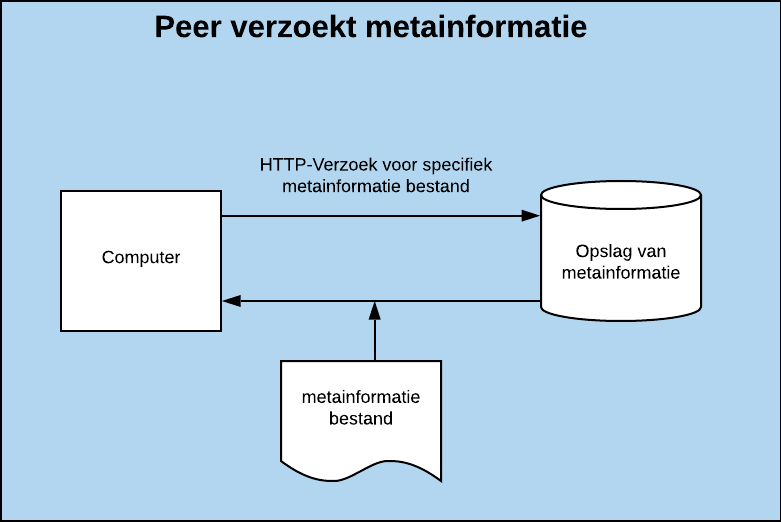
\includegraphics[scale=.4]{torrent-1.png}
\caption[Peer metainformatie stap  - Torrenting 1]{De peer maakt een verzoek aan een opslagplaats voor een metainformatie bestand.}
\end{figure}

Dit metainfo bestand wordt over het algemeen afgehaald van een website of een ftp server. Een gekend voorbeeld van een website die metainfo bestanden ter beschikking stelt is \textit{The pirate bay}. Dit bestand bevat essentiële informatie om de rest van het protocol te faciliteren. Het bevat de namen en bestandsstructuur van de verschillende bestanden binnen deze Torrent. Voor elk van deze bestanden is ook een MD5-Hashwaarde voorzien zodat eenmaal het bestand gedownload is de gebruiker kan controleren of het niet beschadigd is geraakt bij het download proces. Er wordt ook een zogenaamde infowaarde en stuklengte voorzien. Deze komen later aanbod. Het belangrijkste element in het metainfo bestand is echter het IP-adres van de \textbf{Tracker}. Deze Tracker is een computer die de andere delen van het protocol gaat overzien en aansturen. Aangezien er één centrale computer nodig is om dit protocol in goede banen te leiden is er dan ook sprake van een hybride netwerk.\\

\begin{figure}[h!]
	\centering
		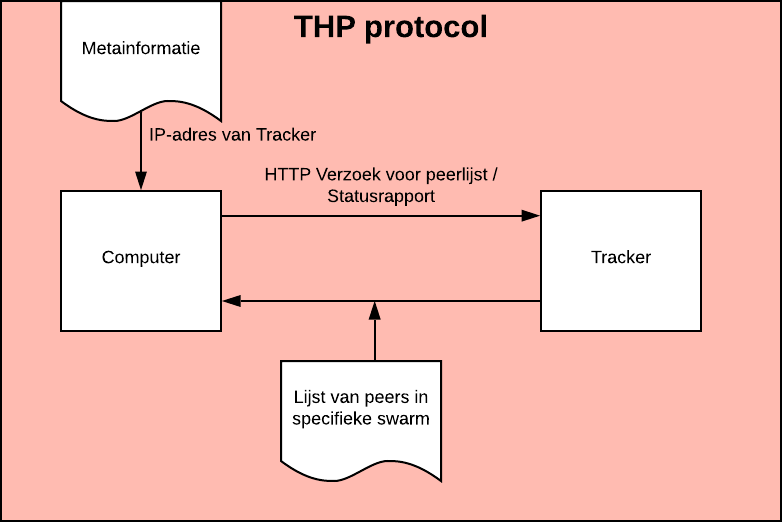
\includegraphics[scale=.4]{torrent-2.png}
			\caption[THP stap - Torrenting 2]{De peer doet een verzoek voor de peerlijst aan de tracker doormiddel van informatie uit het metainformatie bestand.}
\end{figure}
\newpage
Om deze stap te verduidelijken kan er gebruik worden gemaakt van volgend voorbeeld:\\

Bob en Alice maken een Torrent van hun website. Hun website bevat verschillende pagina's en afbeeldingen die zich in een media folder bevinden. Ze stellen een lijst op van deze verschillende bestanden en berekenen voor elk van deze bestanden een MD5-Hash waarde. Bobs computer zal de rest van het protocol coördineren en aldus functioneren als Tracker. Er wordt tot slot een unieke infosleutel voorzien en stuklengte (het is aangeraden deze stuklengte rond 70kb in te stellen). Op basis van deze informatie wordt een metainfo bestand aangemaakt dat wordt beschikbaar gesteld aan de buitenwereld.\\

In de volgende stap wilt men toegang verkrijgen tot andere peers die dit bestand bezitten. Men heeft immers andere computers nodig vanwaar men het bestand kan downloaden. De verzameling van computers die een torrent toegankelijk stellen voor het netwerk wordt ook wel een \textbf{swarm} genoemd. Men kan een swarm dan ook zien als een klein netwerk met als functie toegang te verlenen tot een specifieke collectie van bestanden. De functie van de Tracker is om toegang te verschaffen aan deze Swarm en ook informatie hierover bij te houden. Het principe van toegang verschaffen en informatie bijhouden wordt ook wel \textit{THP}(Tracker HTTP protocol) genoemd. De locatie van deze tracker staat vermeld in het metainfo bestand. Om een lijst van peers te krijgen die in een swarm zit, stuurt de computer een HTTP-GET verzoek naar de tracker. In dit verzoek moeten een aantal zaken worden meegestuurd waaronder het IP-adres van de computer, de infosleutel en de poort waarop de communicatie met andere peers kan gebeuren. De Tracker zal vervolgens aan de hand van de infosleutel een lijst van peers terugsturen die de gegeven bestanden ter beschikking stellen.\\

\begin{figure}[h!]
	\centering
		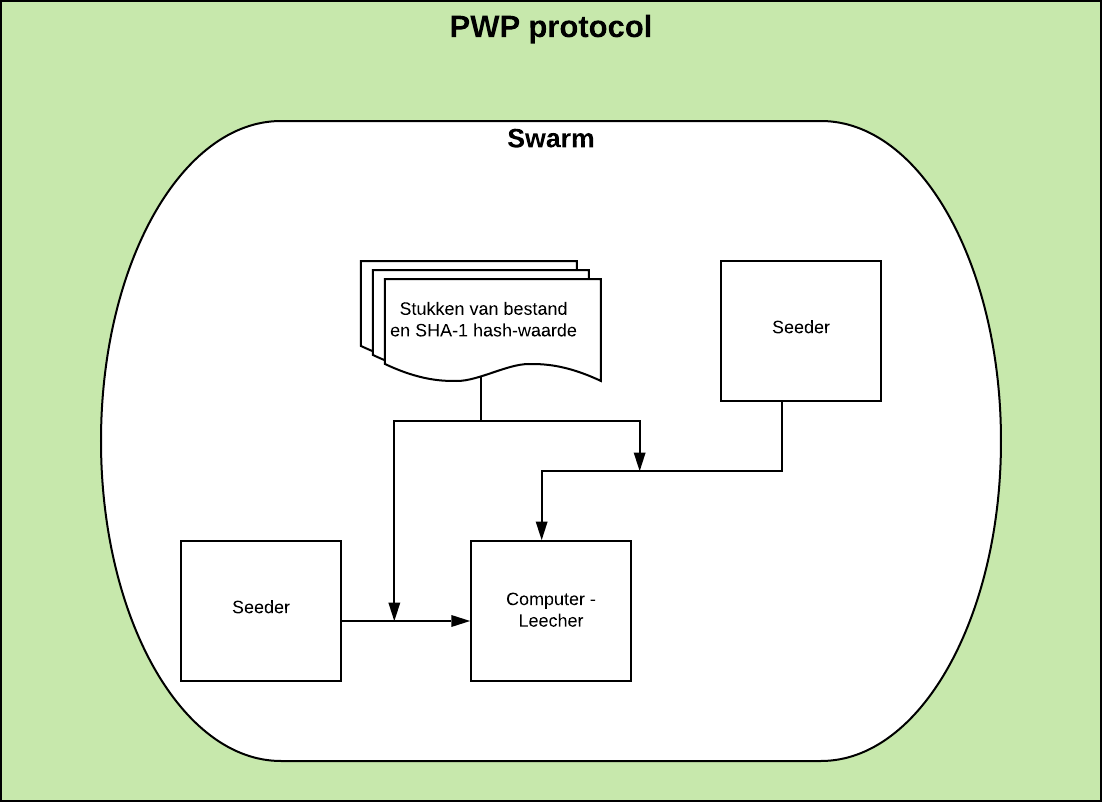
\includegraphics[scale=0.6]{torrent-3.png}
	\caption[PWP stap - Torrenting 3]{De peer verzoekt andere peers voor stukken data en downloadt op die manier de Torrent bestanden.}
\end{figure}
\newpage
Om dit principe te verduidelijken wordt verder gebouwd op bovenstaand voorbeeld:\\

Charlie wil de website van Bob en Alice. Hij heeft van Alice het metainfo bestand ontvangen. Aangezien dit bestand het IP-adres van Bobs computer als Tracker bestempelt wordt er naar deze computer een HTTP-GET verzoek verstuurd. Bob en Alice hebben beiden deze bestanden lokaal staan en vormen aldus samen een swarm. Charlie zal hun IP-adres en poort waarop het verkeer kan verlopen doorgestuurd krijgen en gaat rechtstreeks met beide computers communiceren om de bestanden te downloaden.\\

Opmerking: netwerken en bestanden zijn erg veranderlijk, een computer kan elk moment uitgaan of van het netwerk treden. Het is dus noodzakelijk dat de Tracker een accurate lijst van peers gaat bijhouden in de Swarm. Om dit te bereiken zal een Tracker vragen dat elke peer op een vast tijdsinterval zijn status gaat rapporteren. Zo kan de Tracker accurate informatie voorzien.\\

De computer heeft nu een lijst van verschillende Peers binnen een specifieke swarm. De laatste stap van het protocol is het effectief verkrijgen van de bestanden. De communicatie loopt uitsluitend tussen de verschillende peers zelf. Deze stap wordt ook wel aangeduid als het \textit{PWP} protocol (Peer Wire Message). Bandbreedte en andere beperkingen spelen een grote rol binnen netwerkverkeer. Men wil een peer zo weinig mogelijk belasten. Op die manier stimuleert men de peer om zolang mogelijk op het netwerk te blijven. Het is aldus niet praktisch om volledige bestanden op te vragen van één peer. Stel dat het bestand bijvoorbeeld verschillende gigabytes groot is. Hierdoor zal men het bestand opdelen in verschillende kleine stukken. Deze stukken kunnen individueel worden opgevraagd aan verschillende computers. Op deze manier kan men een bestand van verschillende gigabytes in duizend keer opvragen bij verschillende peers die elk enkele mb doorsturen. De grootte van elk stuk wordt bepaald in het metainfo bestand en staat vastgelegd in de zogenaamde stuklengte. Een ander voordeel van deze fragmentering is dat men individuele stukken kan verifiëren. Elk van deze stukken heeft namelijk zijn eigen SHA-1 hashwaarde. Op die manier kan men gedurende de overdracht van een stuk onmiddellijk nagaan of dit goed is toegekomen en indien er fouten zijn dit klein stuk opnieuw opvragen. Het PWP protocol komt neer op het opvragen en valideren van individuele stukken aan verschillende peers.\footnote{De manier waarop deze stukken worden opgevraagd, ligt buiten de scope van deze bachelorproef. Een goed overzicht wordt gegeven in de tekst van \textcite{Fonseca2005}.} Eenmaal alle stukken zijn gedownload, worden deze samengenomen tot het origineel bestand dat opzijn beurt kan worden gevalideerd aan de hand van MD5.\\

Het Torrent protocol heeft duidelijk een aantal voordelen. Zoals eerder vermeld is het nog steeds relevant hoewel het uit 2002 dateert. Het biedt immers een relatief eenvoudige manier aan om bestanden te downloaden. Door een goede metainformatie indexeringswebsite te gebruiken zoals \textit{The pirate bay} vindt men op eenvoudige wijze de correcte bestanden terug. Dit is bij FTP minder evident.\\

Toch zijn er ook veel technische nadelen verbonden aan het Torrent protocol\footnote{Er zijn ook veel morele implicaties verbonden aan Torrenting maar deze vallen buiten de scope van deze bachelorproef.}:

\begin{itemize}
\item Doordat men gebruik moet maken van een centrale Tracker is er ook één SPOF. Indien de tracker onbereikbaar is dan kan het Torrent protocol niet lang functioneren.\\

\item Het verkrijgen van de metainformatie bestanden is niet evident. Men moet toegang krijgen door middel van een indexeringswebsite of de auteur van de Torrent moet dit bestand doorsturen.\\

\item Volgens \textcite{Thanekar2010} kunnen bestanden permanent verloren gaan. Dit is het geval indien er geen Seeders of volledige kopieën beschikbaar zijn.\\

\item Peers communiceren rechtstreeks met elkaar over TCP. Hiervoor heeft men elkaars IP-adres nodig. Dit leidt er dus toe dat men niet anoniem is bij de download en upload van bestanden.\\

\item Er is weinig stimulans voor een peer die bestanden downloadt om deze ook toegankelijk te stellen voor het netwerk en de rol van Seeder op zich te nemen. Om dit probleem te vermijden wordt een zogenaamde \textit{Tit for tat} beleid gehanteerd. Hierbij kunnen peers enkel bestanden downloaden indien ze effectief ook bijdragen aan de download van anderen.\\

\item Tot slot moet men ook rekening houden dat er geen manier is om volledig te verifiëren wat men downloadt. Men kan nagaan of het bestand hetzelfde is als dat in de metafile. Dit is echter geen garantie dat het bestand veilig is en de relevante informatie bevat. 
\end{itemize}

Vele van deze problemen stellen zich ook in het klassieke Client-Server model.

\subsubsection{Gnutella}
Zoals uitgelegd in \ref{torrenting} is het Bit-Torrent protocol niet volstrekt gedecentraliseerd. Er is immers een centraal component (de Tracker) noodzakelijk om de verbinding tot het netwerk van peers tot stand te brengen. Indien deze centrale component onbereikbaar is kan er geen verbinding tot stand worden gebracht. Om dit probleem te omzeilen moet er aldus een manier zijn om in een volstrekt gedecentraliseerde manier bestanden te gaan delen met elkaar. Hiervoor kan men gebruik maken van Gnutella.\\

Gnutella is een protocol met als doelstelling het verspreiden en toegankelijk stellen van bestanden in een volledig gedecentraliseerd netwerk. Het protocol bereikt dit door het versturen van verschillende types van berichten over een TCP/IP connectie. De uitleg over dit protocol is gebaseerd op de \textit{draft RFC} die wordt onderhouden door \textcite{Klingberg2002}. Om het protocol te kunnen gebruiken zijn er aantal stappen die een peer moet overlopen:

\begin{itemize}
\item De peer ($p_1$) zoekt toegang tot het netwerk doormidden van een connectie aan te gaan met een peer die reeds met netwerk verboden is. Voor de duidelijkheid wordt deze initiële peer bestempelt met het symbool $p_0$ doorheen deze tekst.\\
\item De peer ($p_1$) verkrijgt meer informatie over het netwerk door berichten te versturen aan deze peer ($p_0$).\\
\item De peer $p_1$ gaat connecties aan met andere peers. Vervolgens kan $p_1$ bestanden gaan delen of opvragen aan het netwerk.\\
\item De peer $p_1$ is nu een volwaardig lid van het netwerk en kan andere peers toegang verschaffen. $p_1$ kan aldus de rol van initiële peer $p_0$ op zich nemen.
\end{itemize}

\subsubsection{Verbinden op het netwerk}
Zoals eerder aangehaald moet een peer zich verbinden op het Gnutella netwerk om bestanden te kunnen opvragen. Een peer kan toe treden door 

\subsection{Hoe worden bestanden geïdentificeerd op het netwerk}
Een probleem binnen file sharing is de wijze waarop men bestanden opvraagt. Dit kan het best worden geïllustreerd aan de hand van een voorbeeld.\\

Alice wilt graag een afbeelding van de paashaas. Na het opzoek door middel van een zoek machine vind ze deze afbeeldingen op een gegeven URL. Deze URL is verbonden aan een server die op zijn beurt de afbeelding bevat. Alice kan dus eenvoudigweg de afbeelding daar opvragen. Op een gedecentraliseerd systeem is dit niet evident er is immers geen server waar bestanden ter beschikking staan. De bestanden zitten namelijk verspreid over verschillende computers. Toch moet het systeem instaat zijn om bestanden terug te vinden.\\

Om dit probleem op te lossen wordt er niet naar een specifieke plaats genavigeerd zoals met een URL. Het netwerk wordt rechtstreeks bevraagd voor een bestand. De peers die dit bestand ter beschikking hebben zullen dit bestand doorsturen naar de peer die het heeft opgevraagd. Voor dit principe heeft elk bestand een uniek identificatie nummer nodig. Een bestandsnaam is immers niet uniek.\\

Hiervoor kan men gebruik maken van \textbf{Hashfuncties}. Een hashfunctie is een wiskundige functie die aan een

%%=============================================================================
%% Methodologie
%%=============================================================================

\chapter{\IfLanguageName{dutch}{Methodologie}{Methodology}}
\label{ch:methodologie}

%% TODO: Hoe ben je te werk gegaan? Verdeel je onderzoek in grote fasen, en
%% licht in elke fase toe welke stappen je gevolgd hebt. Verantwoord waarom je
%% op deze manier te werk gegaan bent. Je moet kunnen aantonen dat je de best
%% mogelijke manier toegepast hebt om een antwoord te vinden op de
%% onderzoeksvraag.
\section{Hoe de onderzoeksvraag tot stand is gekomen.}
\label{POC_introduction}
Dit onderzoek ontstond uit een persoonlijke interesse. Internet is een zeer veranderlijk geheel met tal van nieuwe technologieën die ingeburgerd raken. Software ontwikkeling is dan ook geen vast gegeven. Toch zijn er een aantal basis fundamenten waarop softwareontwikkeling gebaseerd is. Een van deze fundamenten is het klassieke server-client model. In dit model voorziet één centrale computer bestanden of diensten voor tal van andere computers. Een gekend voorbeeld hiervan is de manier waarop het internet werkt ook wel bekend onder het HTTP protocol.\\

Bestaat er dan geen alternatief voor het Client-Server model? Distributed Computing tracht deze vraag te beantwoorden. Eén van de oplossingen is een zogenaamd P2P netwerk. Binnen dit type netwerk voorzien computers onderling bestanden en diensten aan elkaar voorzien. Dit type netwerk werd vooral populair onder de vorm van File-Sharing Protocollen. Gekende voorbeelden zijn hierbij Pirate Bay en Napster. Hoewel deze protocollen een eenvoudig en elegant alternatief boden stonden ze nog niet op punt. Zo was er geen manier om op een veilig wijze aan dataopslag te doen.\\

Blockchain bracht een oplossing voor het probleem van dataopslag. Blockchain technologie is vooral bekend van Bitcoin en de financiële impact die deze met zich mee bracht. Toch zijn de implicaties veel diepgaander. Blockchain bied een manier om op een veilige wijze aan dataopslag te doen in een gedistribueerd netwerk. Door dat data integriteit kan gewaarborgd worden kunnen ontwikkelaar veiligere en robuustere oplossingen ontwikkelen voor een P2P netwerk.\\

Toch bleef de blockchain technologie niet beperkt tot Bitcoin en P2P netwerken en werd ze veel verder ontwikkeld. Zo kwam Ethereum met het idee van smart contracts die software ontwikkelaars in staat stellen om transacties op Blockchain netwerken verder te controleren. Hierdoor kunnen applicaties worden ontwikkeld die op een volledig gedistribueerde manier werken. Het is een zeer fascinerende en revolutionaire manier van denken die grote implicaties met zich mee kan dragen.\\

Deze bachelorproef wil deze technologie verkennen en gebruiken in één van de meest fundamentele stappen van moderne software ontwikkeling: versiebeheer.\\

Uiteraard is deze bachelorproef niet het enige onderzoek over het decentraliseren van versiebeheer. In hun onderzoek decentraliseren \textcite{Nizamuddin2019} versiebeheer aan de hand van de Ethereum blockchain en IPFS. Dit is een zeer interessante benadering geweest maar bleef echter beperkt. Veel van de achterliggende concepten werden niet uitgelegd en hun oplossing was eerder beperkt in grote in en complexiteit. Deze bachelorproef wilt hierop een aanvulling bieden en uitleggen wat blockchain, versiebeheer en IPFS exact zijn en hoe deze kunnen worden gecombineerd.

\section{Het ontleden van de onderzoeksvraag.}
\label{ontleden van de onderzoeksvraag}
Zoals besproken in \ref{POC_introduction} is de uiteindelijke onderzoeksvraag waarop een antwoord wordt gezocht: \textbf{Hoe kan men door middel van Blockchain principes en IPFS een werkbaar gedecentraliseerd versiebeheersysteem ontwikkelen} Deze wordt onderverdeeld in verschillende deelvragen die sequentieel zijn beantwoord in de literatuurstudie. Hieronder volgt een kort overzicht en antwoord op de verschillende deelvragen. Voor meer informatie zie \ref{ch:stand-van-zaken}.
 
\begin{table}[h!]
\begin{tabularx}{\linewidth}{ |X|X| }
\hline
Deelvraag & Antwoord \\ \hline
Wat zijn de problemen die versiebeheersystemen oplossen? & 
versiebeheersystemen bieden een manier om verschillende softwareversies aan te maken. Hierdoor kunnen softwareontwikkelaars ten allen tijden toegang krijgen tot verschillende versies van hun software. Versiebeheersystemen stellen ontwikkelaars in staat om hun code op een eenvoudige manier onderling met elkaar te delen en samen te werken.\\ \hline
Waaruit bestaat een versiebeheersysteem? & Een versiebeheersysteem bestaat uit twee delen: Een manier om bestanden op te slaan en te delen met elkaar. Ten tweede een wijze om bestanden te gaan archiveren. Dit wilt zeggen dat ze verschillende versies van de bestanden kunnen opslaan en ook toegang bieden tot deze versies.\\ \hline
Waarom zouden we van gecentraliseerde (server-client architectuur) versiebeheersystemen overstappen naar een gedecentraliseerde variant?         & Moderne versiebeheersystemen zijn vaak het eigendom van grote tech-giganten. Binnen software ontwikkeling streven open-source developers en bedrijven die streven naar democratische softwareontwikkeling. Gedecentraliseerde systemen kaderen goed binnen deze ideologie. Gedecentraliseerde systemen hebben ook het voordeel dat ze geen centraleserver architectuur vereisen. Servers zijn immers kostelijk en mocht de server kapot gaan is men alle gegevens kwijt (\textit{het zogenaamde SPOF probleem}).\\ \hline
Wat zijn de eigenschappen en valkuilen van gedecentraliseerde(P2P) netwerken? & P2P netwerken bieden een manier om op een gedecentraliseerde wijze diensten en software aan te bieden. Elke peer zal hierbij de rol van zowel server als client op zich nemen om dit te bereiken. Het grootste nadeel is echter dat deze netwerken een groot aantal deelnemers vereisen om functioneel werkbaar te zijn.\\ \hline
\end{tabularx}
\end{table} 
\newpage
\newpage
\begin{table}[h!]
\begin{tabularx}{\linewidth}{ |X|X| }
\hline
Deelvraag & Antwoord \\ \hline
Wat is IPFS en hoe kadert het binnen versiebeheer? & IPFS is een P2P file-sharing protocol. Door IPFS kan men op een gedecentraliseerde wijze bestanden gaan opslaan en opvragen. Aangezien versiebeheersystemen toegang willen bieden tot het delen van software versies zijn daar uiteraard ook bestanden bij betrokken. Een softwareproject is immers niets meer of minder dan verschillende bestanden. Hiervoor is IPFS dus een geschikte kanidaat.\\ \hline
Wat zijn smartcontracts en hoe bieden ze een meerwaarde aan Blockchain applicaties? & Smartcontracts is een manier om op een gedecentraliseerde wijze code uit te voeren en de data in de blockchain aan te passen. Zo kan men voorwaarden opleggen aan wijzigingen in de data. Door smartcontracts kan men bijvoorbeeld enkel de eigenaar van bepaalde data toestaan om deze data te wijzigen.\\ \hline
\end{tabularx}
\end{table} 
\newpage
\newpage
Bovenstaande deelvragen bieden een goed overzicht van wat er exact nodig is om een Proof Of Concept op te stelen. De eigenlijke doelstelling van de onderzoeksvraag is het bekomen van een gedecentraliseerd versiebeheer systeem. Welke eigenschappen moet de POC voorzien om te voldoen aan deze vereisten?:

\begin{enumerate}
	\item De oplossing die wordt ontwikkeld mag geen centrale component hebben en moet op een volledig gedistribueerde manier in staat zijn om te functioneren.
	\item De oplossing moet een gebruiker instaat stellen om documenten met anderen te kunnen delen.
	\item De oplossing moet een manier aanbieden om wijzigingen aan deze documenten op te slaan onder de vorm van verschillende versies. Deze verschillende versies moeten kunnen geraadpleegd worden.
\end{enumerate}

\section{Tools}
Het delen van bestanden wordt mogelijk gemaakt door middel van IPFS. Dit protocol stelt de POC in staat om bestanden te verspreiden op een gedistribueerde manier en deze vervolgens opnieuw op te vragen. Hiervoor gebruikt IPFS het principe van een CID. Dit is in essentie een zelfbeschrijvende hash code die vervolgens kan worden gebruikt om bestanden op te halen -zie \ref{ipfs_decent}-. IPFS stelt ons ook in staat om meerdere versies van dezelfde bestand(en) op te slaan en ter beschikking te stellen. neem bijvoorbeeld onderstaand scenario:\\

Bob en Alice willen een website ontwikkelen. Bob plaatst de homepagina op het IPFS netwerk en krijgt een CID om dit bestand opnieuw op te vragen. Hij deelt deze CID met Alice die vervolgens het bestand lokaal binnenhaalt. Alice brengt enkele wijzigingen aan en zet het bestand opnieuw op het netwerk. Alice zal een nieuwe CID worden toegewezen. Er zijn nu in feite twee verschillende versies van dit bestand op het netwerk, een versie van Bob die kan worden opgehaald met de CID die Bob heeft en een versie van Alice met haar eigen CID.\\

Toch is IPFS op zich niet voldoende. Er is immers geen eenvoudige manier voorzien om deze CIDS met elkaar te delen. Hier biedt blockchain een oplossing. Blockchain functioneert immers als een databank. De CIDS kunnen daar dus worden bewaard en opgevraagd. Om dit proces van opslaan en opvragen te vereenvoudigen wordt gebruik gemaakt van smart contracts. Niet iedere blockchain ondersteunt deze smartcontracs. Ethereum is een gekend voorbeeld van een netwerk dat dit wel ondersteunt.\\

Deze smartcontracts worden geschreven in de programmeertaal Solidity. Veel netwerken vragen transactiekosten voor het werken met smartcontracts . Om deze transactie kosten te vermeiden kan er gebruik gemaakt worden van een lokaal Ethereum netwerk. Dit lokaal netwerk voorziet dezelfde functies maar heeft geen transactiekosten. De software die hiervoor gebruik wordt is \textcite{Ganache}.\\

Het ontwikkelen en testen van smartcontracts is ook niet evident. Om dit te vergemakkelijken wordt gebruik gemaakt van de \textcite{Truffle} suite. Deze suite biedt de mogelijkheid om smartcontracts te testen. Hiervoor wordt gebruik gemaakt van het javascript framework Mocha.js. Truffle wordt ook gebruikt om de smartcontracts die worden ontwikkeld op de lokale blockchain uit te rollen.\\

Tot slot wordt er gebruik gemaakt van een console applicatie geschreven in Dotnet-core 3.1 om de verschillende elementen samen te brengen. Deze console applicatie zal onder andere de verschillende bestanden op het IPFS netwerk plaatsen en de smartcontracts op de blockchain aanspreken. Om smartcontracts te kunnen aanspreken vanuit onze console applicatie zal gebruik gemaakt worden van \textcite{Nethereum}. Om IPFS te kunnen gebruiken wordt gebruik gemaakt van \textcite{IPFSClient}.\\

\section{Meetbare criteria}
Zoals hierboven vermeldt wordt -zie \ref{ontleden van de onderzoeksvraag} zijn er drie eigenschappen waaraan het ontwikkelde prototype moet voldoen:

\begin{enumerate}
	\item De oplossing die wordt ontwikkeld mag geen centrale component hebben en moet op een volledig gedistribueerde manier in staat zijn om te functioneren.
	\item De oplossing moet een gebruiker instaat stellen om documenten met anderen te kunnen delen.
	\item De oplossing moet een manier aanbieden om wijzigingen aan deze documenten op te slaan onder de vorm van verschillende versies. Deze verschillende versies moeten kunnen geraadpleegd worden.
\end{enumerate}

Hoe kunnen we deze drie eigenschappen nu concreet af toetsen aan de ontwikkelde oplossing?\\

De oplossing voldoet aan de eerste vereiste als er strikt gebruik maakt van gedecentraliseerde P2P protocollen. Deze protocollen werken namelijk per definitie zonder centraal element. Doorheen de POC wordt gebruik gemaakt van IPFS en de Ethereum blockchain. Beide P2P protocollen. Zolang de console applicatie die deze twee protocollen gaat combineren geen gebruik maakt van een centrale server wordt aldus aan deze vereiste voldaan.\\

Om een functioneel versiebeheersysteem te zijn moet er een manier zijn om documenten te gaan opslaan en opvragen. Het moet ook mogelijk zijn om deze documenten met andere te gaan delen. Concreet is er dus aan de vereiste gedaan als volgende drie functionaliteiten zijn geïmplementeerd:

\begin{enumerate}
\item Een manier om bestanden te gaan opslaan binnen de oplossing.
\item Een manier om opgeslagen bestanden opnieuw te gaan downloaden.
\item Een manier om deze opgeslagen bestanden te gaan delen met iemand anders.
\end{enumerate}

De laatste vereiste stelt dat er een manier moet zijn om wijzigingen aan te brengen aan de bestanden. Deze wijzigingen worden opgeslagen onder de vorm van verschillende versies. Het moet tevens mogelijk zijn om terug te gaan naar een eerdere versie van een bestand. Dat wilt concreet zeggen dat het mogelijk moet zijn om terug te grijpen naar een eerdere versie van het bestand voor een bepaalde wijziging is aangebracht. Er wordt dus aan de vereiste voldaan indien volgende functionaliteit aanwezig is:

\begin{enumerate}
\item Er kunnen wijzigingen worden aangebracht aan de bestanden binnen de oplossing.
\item Deze wijzigingen moeten publiekelijk toegankelijk zijn. Dat wilt concreet zeggen dat andere deze wijzigingen moeten kunnen raadplegen.
\item Er moet een mogelijkheid voorzien worden om terug te grijpen naar een eerdere versie van de bestanden. 
\end{enumerate}

\textbf{Indien aan al deze vereiste wordt voldaan kan men spreken van een werkbaar gedecentraliseerd versiebeheersysteem.}\\

Al deze vereisten kunnen worden samengevat in onderstaande tabel:
\begin{table}[h!]
	\centering
	\begin{tabular}{ |p{14cm}|}
 		\hline
 		\large \textbf{Succescriteria van de POC} \\
 		\hline
 		De applicatie mag enkel gebruik maken van P2P protocollen, deze zijn per definitie gedecentraliseerd. Er mag aldus geen centrale component gebruikt worden.\\
 		\hline 
 		Men moet instaat zijn om bestanden te gaan opslaan binnen de applicatie op een gedecentraliseerde manier.\\
 		\hline
 		De opgeslagen bestanden moeten opnieuw gedownload kunnen worden.\\
 		\hline
		Deze bestanden moeten eveneens kunnen worden gedeeld met anderen.\\
 		\hline
 		Er moeten wijzigingen kunnen worden aangebracht binnen deze bestanden. Deze moeten kunnen worden opgeslagen door het systeem.\\
 		\hline
 		Andere die dit bestand lokaal hebben gedownload moeten instaat zijn om deze wijzigingen binnen te halen en hun eigen wijzigingen aanbrengen.\\
 		\hline
 		Er moet een manier voorzien worden waarop men terug kan grijpen naar een eerder versie van het bestand.\\
 		\hline
 	\end{tabular}
	\label{tbl_concepts}
	\caption{Succescriteria van de POC.}
\end{table}
\newpage
\section{Werkwijze}
Om de verschillende smartcontracts te ontwikkelen is er gekozen om gebruik te maken van een klasse diagram. Dit diagram biedt een schematisch overzicht van de verschillende contracten die ontwikkeld zijn alsook de verschillende functies en attributen

\textbf{TODO: Hier komt nog een klasse diagram alsook een kort overzicht van de oplossing}

\section{Bedenkingen}

% Voeg hier je eigen hoofdstukken toe die de ``corpus'' van je bachelorproef
% vormen. De structuur en titels hangen af van je eigen onderzoek. Je kan bv.
% elke fase in je onderzoek in een apart hoofdstuk bespreken.

%\input{...}
%\input{...}
%...

%%=============================================================================
%% Conclusie
%%=============================================================================

\chapter{Conclusie}
\label{ch:conclusie}

\textbf{Dit zijn mijn conclusies in bulletpoints die verder zullen worden verwerkt tot een doorlopende tekst:}
\begin{enumerate}
\item Het ontwikkelen van een versiebeheersysteem door middel van Blockchain en IPFS is technisch haalbaar. 
\item Ik heb hierbij gekozen voor het Ethereum netwerk aangezien dit het meest gedocumenteerde netwerk is.
\item Door de hoge transactie kosten die verbonden zijn aan het Ethereum netwerk is de oplossing te duur. Vooral aangezien de alternatieve gratis zijn.
\item Er bestaan ook netwerken zonder transactiekosten maar door dat deze minder gebruikt worden en het aantal participanten klein is nemen de transacties veel tijd in beslag.
\item Blockchain is een interesante technologie en door de volledig gedecentraliseerde organisatie ideologisch mooi maar het is financieel niet haalbaar.
\end{enumerate}



%%=============================================================================
%% Bijlagen
%%=============================================================================

\appendix
\renewcommand{\chaptername}{Appendix}

%%---------- Onderzoeksvoorstel -----------------------------------------------

\chapter{Appendix}
{\Huge Appendix 1: Onderzoeksvoorstel}\\
Het onderwerp van deze bachelorproef is gebaseerd op een onderzoeksvoorstel dat vooraf werd beoordeeld door de promotor. Dat voorstel is opgenomen in deze bijlage.

% Verwijzing naar het bestand met de inhoud van het onderzoeksvoorstel
%---------- Inleiding ---------------------------------------------------------

\section{Introductie} % The \section*{} command stops section numbering
\label{sec:introductie}

De onderzoeksvraag waaruit wordt vertrokken luidt als volgt: \textbf{"Hoe kunnen we doormiddel van IPFS en Blockchain technologie versiebeheer van een Client-Server architectuur naar een gedecentraliseerde Peer-to-peer model overzetten?"} Binnen deze onderzoeksvraag zijn er vier begrippen:\\\\
\begin{itemize}
\item \textbf{Versiebeheer}: Git -een grote speler op het gebied van Versiebeheer- hanteert volgende definitie van het begrip “Versiebeheer is het systeem waarin veranderingen in een bestand of groep van bestanden over de tijd wordt bijgehouden, zodat je later specifieke versies kan opvragen.” Deze definitie werd gepubliceerd in het boek \textit{Pro git} \autocite{Chacon2014}. \\\\

\item \textbf{IPFS}: Interplanetary File System of (IPFS)werd in de paper “IPFS - Content Addressed, Versioned, P2P File System” geïntroduceerd door \textcite{Benet2014}. Hierin stelde hij zijn technologie voor als een peer-to-peer gedistribueerd bestandssysteem waarin alle computers werken met dezelfde bestandsindeling. Hiermee wordt bedoeld dat bestanden kunnen worden opgedeeld in verschillende delen (\textit{ook wel 'Shards' genoemd}) en vervolgens worden opgeslagen op verschillende computers op een gezamenlijk netwerk. Vervolgens kunnen bestanden worden opgevraagd door middel van dit gezamenlijk netwerk aan te spreken. Er is dus geen gecentraliseerd aanspreekpunt.\\\\

\item \textbf{Blockchain}: Blockchain is een manier om data op te slaan aan de hand van blokken. Deze blokken bevatten verschillende gegevens. Deze gegevens worden omgezet door middel van wiskundige functies die ook wel hashfuncties worden genoemd. Door de blokken onderling aan elkaar te koppelen en wiskundige functies te gebruiken bij het verifiëren van de integriteit van de blokken ontstaat er een veilige en volledig gedecentraliseerde manier van dataopslag.\\\\

\item \textbf{P2P}: Tot slot is er ook het concept van Peer-to-peer (courant afgekort als P2P). Voor een gangbare definitie kan gebruik gemaakt worden van de werken van \textcite{Schollmeier2001} en \textcite{IAB5694}. Hierbij wordt gesteld dat P2P bestaat uit verschillende computers (nodes) die onderling met elkaar verbonden zijn. Deze nodes vervullen daarbij de rol van zowel server als client (zogenaamde Servents). Hierdoor kunnen de verschillende nodes diensten en data aan elkaar opvragen en delen zonder een centraal aanspreekpunt (client-server architectuur). Dit is dan ook het achterliggende principe van IPFS. Blockchain is een manier om gegevens~ en gedragsintegriteit (als gedefinieerd in \autocite{Drescher2017}) te waarborgen zonder centrale autoriteit binnen P2P netwerken.\\
\end{itemize}

\noindent Versiebeheer wordt vaak uitbesteed aan derden of zelf gedaan aan de hand van een centrale server. Het nadeel hiervan is dat er één centrale plek is waar het kan mislopen. Stel bijvoorbeeld dat de centrale server gegevens verliest is men alles kwijt. Een ander probleem is dat er binnen versiebeheer een aantal monopolies ontstaan waaronder Microsoft die GitHub kocht in 2018.  Dit staat haaks op de open source beweging die streeft naar een transparante en democratische manier van software ontwikkeling. Door het introduceren van de bovengenoemde technologieën kunnen zowel de bestanden als de nodige informatie voor versiebeheer worden verspreid waardoor er geen centraal punt is en er ook geen commercieel bedrijf bij betrokken is.\\

\noindent De doelstelling van dit onderzoek is om versiebeheer te decentraliseren. Daaronder wordt verstaan overstappen van de klassieke server-client architectuur zoals github (of een lokaal gehost versiebeheer systeem) naar een P2P netwerk. Voor de bestanden wordt gebruik gemaakt van de reeds bestaande IPFS technologie. Hierbij zal een blockchain oplossing worden ontwikkeld om het geheel te ondersteunen (metadata, manifest bestanden,...). -Zie ook \ref{sec:methodologie} Methodologie.-\\

\noindent Om de onderzoeksvraag volledig te beantwoorden kan deze nog verder opgesplitst worden in verschillende deelvragen. Deze vragen komen dan ook chronologisch aan bod om uiteindelijk tot een werkend systeem te bekomen. De verschillende deelvragen die worden behandeld zijn:

\begin{itemize}
\item{Wat zijn de problemen van versiebeheer binnen softwareontwikkeling en hoe worden deze aangepakt door versiebeheer systemen zoals GIT?}
\item{Waarom zouden we van gecentraliseerde (server-client architectuur) versiebeheer systemen overstappen naar een gedecentraliseerde variant?}
\item{Wat zijn de eigenschappen en valkuilen van gedecentraliseerde (P2P) netwerken?}
\item{Hoe gaan protocollen zoals Gnutella en BitTorrent te werk voor Peer-to-peer filesharing?}
\item{Wat is IPFS en hoe vergelijkt het met andere gedecentraliseerde filesharing protocollen?}
\item{Op welke manier biedt IPFS een meerwaarde ten opzichte van klassieke versiebeheer systemen?}
\item{Wat zijn de basisprincipes van Blockchain?}
\item{Hoe kunnen data veilig en integer worden bewaard op een Blockchain netwerk?}
\item{Welke meerwaarde kan blockchain bieden binnen de context van Peer-to-peer netwerken?}
\item{Wat zijn smartcontracts en hoe kunnen ze een meerwaarde bieden binnen blockchain oplossingen? }
\item{Op welke wijze kunnen we IPFS en blockchain combineren tot een werkzaam versiebeheer systeem?}
\end{itemize}

%---------- Stand van zaken ---------------------------------------------------

\section{State-of-the-art}
\label{sec:state-of-the-art}

De manier van werken is gebaseerd op het artikel “Decentralized document version control using ethereum blockchain and IPFS.” \autocite{Nizamuddin2019} In het onderzoek wordt er gebruik gemaakt van smart contracts. Dit is in essentie code die zal uitgevoerd worden als aan bepaalde voorwaarden wordt voldaan. Deze smart contracts worden gebruikt om de verschillende aspecten van versiebeheer en data vast te leggen en uit te voeren. Voor de bestanden binnen het project wordt gekozen voor IPFS om op een gedecentraliseerde manier deze te kunnen opslaan. \\\\
De paper vormt een zeer goede aanzet en ook de werkmethode is uitvoerig beschreven. Toch blijft het zeer abstract. Belangrijke aspecten van versiebeheer worden kort of niet aangehaald waaronder “cloning”, “merging” of “branching”. In de bovengenoemde paper wordt een sterke focus op Ethereum gelegd, ontwikkeling bovenop deze blockchain interpretatie brengt echter significante overhead met zich mee. Zo is de snelheid van het systeem afhankelijk van de capaciteit en belasting van het netwerk op het gegeven moment.\\\\
Deze bachelorproef legt de focus op het ontwikkelen van een concrete toepassing. Ook de meer complexe en technische problemen zullen worden behandeld. De algemene principes van blockchain zullen vrijer worden geïmplementeerd en op een lokaal netwerk van enkele computer worden verspreid. In plaats van een grotere architectuur en implementatie te gebruiken
% Voor literatuurverwijzingen zijn er twee belangrijke commando's:
% \autocite{KEY} => (Auteur, jaartal) Gebruik dit als de naam van de auteur
%   geen onderdeel is van de zin.
% \textcite{KEY} => Auteur (jaartal)  Gebruik dit als de auteursnaam wel een
%   functie heeft in de zin (bv. ``Uit onderzoek door Doll & Hill (1954) bleek
%   ...'')


%---------- Methodologie ------------------------------------------------------
\section{Methodologie}
\label{sec:methodologie}

Er wordt vertrokken vanuit een literatuurstudie om de verschillende elementen van versiebeheer en de reeds bestaande technologieën te verkennen. Vervolgens komen de aspecten van blockchain en IPFS aan bod door middel van een demo waarin wordt gebruik gemaakt van een Word document met verschillende versies.\\\\
Tot slot worden de verschillende aspecten van versiebeheer aan de hand van een demo-applicatie geïllustreerd. Hiervoor zijn er drie hypothetische gebruikers: Alice, Bob en Carol die samen een T-shirt webshop ontwikkelen. Ze zullen hiervoor gebruiken maken van ASP.Net en Visual Studio. Binnen hun ontwikkelingsproces zullen ze een aantal gekende problemen tegenkomen waaronder “merge conflicten” en verschillende “branches”.\\\\
Bij elk van die problemen wordt er gekeken naar hoe Git -een klassiek versiebeheer systeem- dit oplost en hoe er een oplossing kan voorzien worden vanuit de voorgestelde gedistribueerde blockchain benadering. Voor het opstellen van de blockchain wordt gebruik gemaakt van C\# en Nethereum \autocite{Nethereum}. Aangezien er wordt gesteund op de IPFS API wordt er gebruik gemaakt van de open source bibliotheek net-ipfs-client-http geschreven door \textcite{IPFSClient}. De bedoeling is om op het einde van de bachelorproef tot een werkend prototype te komen dat gebruikt kan worden voor verschillende doeleinden.

%---------- Verwachte resultaten ----------------------------------------------
\section{Verwachte resultaten}
\label{sec:verwachte_resultaten}

Het eindresultaat van de Bachelorproef is om op een onderbouwde manier een prototype aan te reiken om op gedecentraliseerde wijze aan versie beheer te gaan doen. De voorgestelde werkwijze wordt grondig vergeleken met Git op de volgende twee punten:\\\\

\begin{itemize}
\item Snelheid van een transactie: hoe lang duurt het om bewerkingen zoals pull requests en branching toe te passen op een project en/of branch?
\item Performantie qua geheugengebruik: hoe efficiënt wordt er binnen de algoritmen van de oplossing omgesprongen met geheugengebruik? Hiermee wordt zowel het extern geheugen (Hardeschijf, SSD) als het werkgeheugen bedoelt.\\\\
\end{itemize}

\noindent De verwachting is dat de implementatiesnelheid lager zal zijn dan met de klassieke Git-systemen, omdat blockchain van nature vrij omslachtig en intensief is. De performantie van het geheugensysteem zal eveneens slechter scoren ten opzichte van Git. De blockchain implementatie waarborgt echter een hogere mate van data integriteit .  

%---------- Verwachte conclusies ----------------------------------------------
\section{Verwachte conclusies}
\label{sec:verwachte_conclusies}

Gedecentraliseerd versiebeheer door middel van Blockchain en IPFS is zeker technisch mogelijk. De voordelen die het biedt zijn niet alleen zuiver ideologisch.De inherente garantie op data integriteit en het weghalen van een centraal ``\textit{point of failure}'' is interessant voor grote bedrijven met een groot aantal aan verschillende projecten. Er zijn echter een aantal nadelen verbonden waaronder de omslachtige procedure en het intensief gebruik van computertechnische middelen. Dit maakt het voor kleine bedrijven minder interessant.

%%---------- Andere bijlagen --------------------------------------------------
%\input{...}
\newpage
{\Huge Appendix 2: Voorbeeld RCS}\\
\label{ch:voorbeeld-rcs}
\graphicspath{{../../../Images/}} 

%%---------- Referentielijst --------------------------------------------------

\printbibliography[heading=bibintoc]

\end{document}
